\documentclass[twoside]{book}

% Packages required by doxygen
\usepackage{fixltx2e}
\usepackage{calc}
\usepackage{doxygen}
\usepackage[export]{adjustbox} % also loads graphicx
\usepackage{graphicx}
\usepackage[utf8]{inputenc}
\usepackage{makeidx}
\usepackage{multicol}
\usepackage{multirow}
\PassOptionsToPackage{warn}{textcomp}
\usepackage{textcomp}
\usepackage[nointegrals]{wasysym}
\usepackage[table]{xcolor}

% Font selection
\usepackage[T1]{fontenc}
\usepackage[scaled=.90]{helvet}
\usepackage{courier}
\usepackage{amssymb}
\usepackage{sectsty}
\renewcommand{\familydefault}{\sfdefault}
\allsectionsfont{%
  \fontseries{bc}\selectfont%
  \color{darkgray}%
}
\renewcommand{\DoxyLabelFont}{%
  \fontseries{bc}\selectfont%
  \color{darkgray}%
}
\newcommand{\+}{\discretionary{\mbox{\scriptsize$\hookleftarrow$}}{}{}}

% Page & text layout
\usepackage{geometry}
\geometry{%
  a4paper,%
  top=2.5cm,%
  bottom=2.5cm,%
  left=2.5cm,%
  right=2.5cm%
}
\tolerance=750
\hfuzz=15pt
\hbadness=750
\setlength{\emergencystretch}{15pt}
\setlength{\parindent}{0cm}
\setlength{\parskip}{3ex plus 2ex minus 2ex}
\makeatletter
\renewcommand{\paragraph}{%
  \@startsection{paragraph}{4}{0ex}{-1.0ex}{1.0ex}{%
    \normalfont\normalsize\bfseries\SS@parafont%
  }%
}
\renewcommand{\subparagraph}{%
  \@startsection{subparagraph}{5}{0ex}{-1.0ex}{1.0ex}{%
    \normalfont\normalsize\bfseries\SS@subparafont%
  }%
}
\makeatother

% Headers & footers
\usepackage{fancyhdr}
\pagestyle{fancyplain}
\fancyhead[LE]{\fancyplain{}{\bfseries\thepage}}
\fancyhead[CE]{\fancyplain{}{}}
\fancyhead[RE]{\fancyplain{}{\bfseries\leftmark}}
\fancyhead[LO]{\fancyplain{}{\bfseries\rightmark}}
\fancyhead[CO]{\fancyplain{}{}}
\fancyhead[RO]{\fancyplain{}{\bfseries\thepage}}
\fancyfoot[LE]{\fancyplain{}{}}
\fancyfoot[CE]{\fancyplain{}{}}
\fancyfoot[RE]{\fancyplain{}{\bfseries\scriptsize Generated by Doxygen }}
\fancyfoot[LO]{\fancyplain{}{\bfseries\scriptsize Generated by Doxygen }}
\fancyfoot[CO]{\fancyplain{}{}}
\fancyfoot[RO]{\fancyplain{}{}}
\renewcommand{\footrulewidth}{0.4pt}
\renewcommand{\chaptermark}[1]{%
  \markboth{#1}{}%
}
\renewcommand{\sectionmark}[1]{%
  \markright{\thesection\ #1}%
}

% Indices & bibliography
\usepackage{natbib}
\usepackage[titles]{tocloft}
\setcounter{tocdepth}{3}
\setcounter{secnumdepth}{5}
\makeindex

% Hyperlinks (required, but should be loaded last)
\usepackage{ifpdf}
\ifpdf
  \usepackage[pdftex,pagebackref=true]{hyperref}
\else
  \usepackage[ps2pdf,pagebackref=true]{hyperref}
\fi
\hypersetup{%
  colorlinks=true,%
  linkcolor=blue,%
  citecolor=blue,%
  unicode%
}

% Custom commands
\newcommand{\clearemptydoublepage}{%
  \newpage{\pagestyle{empty}\cleardoublepage}%
}

\usepackage{caption}
\captionsetup{labelsep=space,justification=centering,font={bf},singlelinecheck=off,skip=4pt,position=top}

%===== C O N T E N T S =====

\begin{document}

% Titlepage & ToC
\hypersetup{pageanchor=false,
             bookmarksnumbered=true,
             pdfencoding=unicode
            }
\pagenumbering{roman}
\begin{titlepage}
\vspace*{7cm}
\begin{center}%
{\Large Human Obstacle Detector \\[1ex]\large 1.\+0 }\\
\vspace*{1cm}
{\large Generated by Doxygen 1.8.11}\\
\end{center}
\end{titlepage}
\clearemptydoublepage
\tableofcontents
\clearemptydoublepage
\pagenumbering{arabic}
\hypersetup{pageanchor=true}

%--- Begin generated contents ---
\chapter{Class Index}
\section{Class List}
Here are the classes, structs, unions and interfaces with brief descriptions\+:\begin{DoxyCompactList}
\item\contentsline{section}{\hyperlink{classDataLoader}{Data\+Loader} \\*Class \hyperlink{classDataLoader}{Data\+Loader} The class \hyperlink{classDataLoader}{Data\+Loader} reads data from files for training purposes and creates H\+OG feature for every image }{\pageref{classDataLoader}}{}
\item\contentsline{section}{\hyperlink{classDetectHuman}{Detect\+Human} \\*Class \hyperlink{classDetectHuman}{Detect\+Human} The class \hyperlink{classDetectHuman}{Detect\+Human} uses a trained S\+VM model to detect humans in an image and returns the pixel coordinates of the bounding boxes containing humans in an image }{\pageref{classDetectHuman}}{}
\item\contentsline{section}{\hyperlink{classTrainSVM}{Train\+S\+VM} \\*Class \hyperlink{classTrainSVM}{Train\+S\+VM} The class \hyperlink{classTrainSVM}{Train\+S\+VM} trains S\+VM using data from class \hyperlink{classDataLoader}{Data\+Loader} and returns the trained data into a X\+ML file }{\pageref{classTrainSVM}}{}
\item\contentsline{section}{\hyperlink{classVisionInput}{Vision\+Input} \\*Class \hyperlink{classVisionInput}{Vision\+Input} The class \hyperlink{classVisionInput}{Vision\+Input} gives different functionalities to use H\+OG feature based Human detection, so that it can be used with live videos from camera sensor or saved videos and image files }{\pageref{classVisionInput}}{}
\end{DoxyCompactList}

\chapter{File Index}
\section{File List}
Here is a list of all documented files with brief descriptions\+:\begin{DoxyCompactList}
\item\contentsline{section}{app/\hyperlink{DataLoader_8cpp}{Data\+Loader.\+cpp} \\*\hyperlink{classDataLoader}{Data\+Loader} method implementation }{\pageref{DataLoader_8cpp}}{}
\item\contentsline{section}{app/\hyperlink{DetectHuman_8cpp}{Detect\+Human.\+cpp} \\*\hyperlink{classDetectHuman}{Detect\+Human} Class declaration  Implementation of class methods to detect humans using an S\+VM model trained on H\+OG features }{\pageref{DetectHuman_8cpp}}{}
\item\contentsline{section}{app/\hyperlink{TrainSVM_8cpp}{Train\+S\+V\+M.\+cpp} \\*\hyperlink{classTrainSVM}{Train\+S\+VM} Class declaration  Implementation of class methods to train S\+VM using data from class \hyperlink{classDataLoader}{Data\+Loader} }{\pageref{TrainSVM_8cpp}}{}
\item\contentsline{section}{app/\hyperlink{VisionInput_8cpp}{Vision\+Input.\+cpp} \\*\hyperlink{classVisionInput}{Vision\+Input} Class declaration  Implementation of class methods to train S\+VM using data from class \hyperlink{classDataLoader}{Data\+Loader} }{\pageref{VisionInput_8cpp}}{}
\item\contentsline{section}{include/\hyperlink{DataLoader_8hpp}{Data\+Loader.\+hpp} \\*\hyperlink{classDataLoader}{Data\+Loader} Class declaration  Declared functions Class to read data from files }{\pageref{DataLoader_8hpp}}{}
\item\contentsline{section}{include/\hyperlink{DetectHuman_8hpp}{Detect\+Human.\+hpp} \\*\hyperlink{classDetectHuman}{Detect\+Human} Class declaration  Declared functions Class to detect humans using an S\+VM model trained on H\+OG features }{\pageref{DetectHuman_8hpp}}{}
\item\contentsline{section}{include/\hyperlink{TrainSVM_8hpp}{Train\+S\+V\+M.\+hpp} \\*\hyperlink{classTrainSVM}{Train\+S\+VM} Class declaration  Declared functions Class to train S\+VM using data from class \hyperlink{classDataLoader}{Data\+Loader} }{\pageref{TrainSVM_8hpp}}{}
\item\contentsline{section}{include/\hyperlink{VisionInput_8hpp}{Vision\+Input.\+hpp} \\*\hyperlink{classVisionInput}{Vision\+Input} Class declaration  Declared functions Class to get data for realtime detection }{\pageref{VisionInput_8hpp}}{}
\item\contentsline{section}{test/\hyperlink{DataLoaderTest_8cpp}{Data\+Loader\+Test.\+cpp} \\*Test cases for \hyperlink{classDataLoader}{Data\+Loader} class methods }{\pageref{DataLoaderTest_8cpp}}{}
\item\contentsline{section}{test/\hyperlink{DetectHumanTest_8cpp}{Detect\+Human\+Test.\+cpp} \\*Test cases for \hyperlink{classVisionInput}{Vision\+Input} class methods }{\pageref{DetectHumanTest_8cpp}}{}
\item\contentsline{section}{test/\hyperlink{TrainSVMTest_8cpp}{Train\+S\+V\+M\+Test.\+cpp} \\*Test cases for \hyperlink{classTrainSVM}{Train\+S\+VM} class methods }{\pageref{TrainSVMTest_8cpp}}{}
\item\contentsline{section}{test/\hyperlink{VisionInputTest_8cpp}{Vision\+Input\+Test.\+cpp} \\*Test cases for \hyperlink{classVisionInput}{Vision\+Input} class methods }{\pageref{VisionInputTest_8cpp}}{}
\end{DoxyCompactList}

\chapter{Class Documentation}
\hypertarget{classDataLoader}{}\doxysection{Data\+Loader Class Reference}
\label{classDataLoader}\index{DataLoader@{DataLoader}}


class \mbox{\hyperlink{classDataLoader}{Data\+Loader}} The class \mbox{\hyperlink{classDataLoader}{Data\+Loader}} captures image/video from camera sensor or files and creates H\+OG feature for every image.  




{\ttfamily \#include $<$Data\+Loader.\+hpp$>$}

\doxysubsection*{Public Member Functions}
\begin{DoxyCompactItemize}
\item 
\mbox{\hyperlink{classDataLoader_a1e3bfa6d0116f0ecc8ec4596e35a09f0}{Data\+Loader}} ()
\begin{DoxyCompactList}\small\item\em constructor \mbox{\hyperlink{classDataLoader}{Data\+Loader}} \end{DoxyCompactList}\item 
cv\+::\+Mat \mbox{\hyperlink{classDataLoader_ae03c549909bc20eb93556ec880fc0cb3}{create\+H\+OG}} (cv\+::\+Mat input\+Image)
\begin{DoxyCompactList}\small\item\em Function to create H\+OG features. \end{DoxyCompactList}\item 
cv\+::\+Mat \mbox{\hyperlink{classDataLoader_a5368b3a970f681058ff7ac92d6d695cb}{load\+Image}} (std\+::string image\+Name)
\begin{DoxyCompactList}\small\item\em Function to load images. \end{DoxyCompactList}\item 
cv\+::\+Mat \mbox{\hyperlink{classDataLoader_a3e6681a241f7a439aaea6b3ffdcbc301}{Camera}} (int camera\+Code)
\begin{DoxyCompactList}\small\item\em Function to read data from camera sensor. \end{DoxyCompactList}\item 
std\+::vector$<$ cv\+::\+Mat $>$ \mbox{\hyperlink{classDataLoader_afc169b8783dac0eba51db8d9114ee9e7}{load\+Video}} (std\+::string video\+File\+Name)
\begin{DoxyCompactList}\small\item\em Function to load video from a video file. \end{DoxyCompactList}\item 
std\+::vector$<$ cv\+::\+Mat $>$ \mbox{\hyperlink{classDataLoader_aa041f12b158eeb0e392052dc4a6c14cc}{load\+From\+Directory}} (std\+::string directory\+Name)
\begin{DoxyCompactList}\small\item\em Function to load all the images from a directory. \end{DoxyCompactList}\item 
\mbox{\hyperlink{classDataLoader_a30951bb663d7a5ff79a4443de0f943ed}{$\sim$\+Data\+Loader}} ()
\begin{DoxyCompactList}\small\item\em destructor \mbox{\hyperlink{classDataLoader}{Data\+Loader}} \end{DoxyCompactList}\end{DoxyCompactItemize}


\doxysubsection{Detailed Description}
class \mbox{\hyperlink{classDataLoader}{Data\+Loader}} The class \mbox{\hyperlink{classDataLoader}{Data\+Loader}} captures image/video from camera sensor or files and creates H\+OG feature for every image. 

\doxysubsection{Constructor \& Destructor Documentation}
\mbox{\Hypertarget{classDataLoader_a1e3bfa6d0116f0ecc8ec4596e35a09f0}\label{classDataLoader_a1e3bfa6d0116f0ecc8ec4596e35a09f0}} 
\index{DataLoader@{DataLoader}!DataLoader@{DataLoader}}
\index{DataLoader@{DataLoader}!DataLoader@{DataLoader}}
\doxysubsubsection{\texorpdfstring{DataLoader()}{DataLoader()}}
{\footnotesize\ttfamily Data\+Loader\+::\+Data\+Loader (\begin{DoxyParamCaption}{ }\end{DoxyParamCaption})}



constructor \mbox{\hyperlink{classDataLoader}{Data\+Loader}} 


\begin{DoxyParams}{Parameters}
{\em none} & \\
\hline
\end{DoxyParams}
\begin{DoxyReturn}{Returns}
none 
\end{DoxyReturn}
\mbox{\Hypertarget{classDataLoader_a30951bb663d7a5ff79a4443de0f943ed}\label{classDataLoader_a30951bb663d7a5ff79a4443de0f943ed}} 
\index{DataLoader@{DataLoader}!````~DataLoader@{$\sim$DataLoader}}
\index{````~DataLoader@{$\sim$DataLoader}!DataLoader@{DataLoader}}
\doxysubsubsection{\texorpdfstring{$\sim$DataLoader()}{~DataLoader()}}
{\footnotesize\ttfamily Data\+Loader\+::$\sim$\+Data\+Loader (\begin{DoxyParamCaption}{ }\end{DoxyParamCaption})}



destructor \mbox{\hyperlink{classDataLoader}{Data\+Loader}} 


\begin{DoxyParams}{Parameters}
{\em none} & \\
\hline
\end{DoxyParams}
\begin{DoxyReturn}{Returns}
none 
\end{DoxyReturn}


\doxysubsection{Member Function Documentation}
\mbox{\Hypertarget{classDataLoader_a3e6681a241f7a439aaea6b3ffdcbc301}\label{classDataLoader_a3e6681a241f7a439aaea6b3ffdcbc301}} 
\index{DataLoader@{DataLoader}!Camera@{Camera}}
\index{Camera@{Camera}!DataLoader@{DataLoader}}
\doxysubsubsection{\texorpdfstring{Camera()}{Camera()}}
{\footnotesize\ttfamily cv\+::\+Mat Data\+Loader\+::\+Camera (\begin{DoxyParamCaption}\item[{int}]{camera\+Code }\end{DoxyParamCaption})}



Function to read data from camera sensor. 


\begin{DoxyParams}{Parameters}
{\em camera\+Code} & of type int \\
\hline
\end{DoxyParams}
\begin{DoxyReturn}{Returns}
image of type cv\+::\+Mat The following function takes image from camera and returns image. Camera code defines which camera sensor\textquotesingle{}s data you want to read 
\end{DoxyReturn}
\mbox{\Hypertarget{classDataLoader_ae03c549909bc20eb93556ec880fc0cb3}\label{classDataLoader_ae03c549909bc20eb93556ec880fc0cb3}} 
\index{DataLoader@{DataLoader}!createHOG@{createHOG}}
\index{createHOG@{createHOG}!DataLoader@{DataLoader}}
\doxysubsubsection{\texorpdfstring{createHOG()}{createHOG()}}
{\footnotesize\ttfamily cv\+::\+Mat Data\+Loader\+::create\+H\+OG (\begin{DoxyParamCaption}\item[{cv\+::\+Mat}]{input\+Image }\end{DoxyParamCaption})}



Function to create H\+OG features. 


\begin{DoxyParams}{Parameters}
{\em input\+Image} & of type cv\+::\+Mat \\
\hline
\end{DoxyParams}
\begin{DoxyReturn}{Returns}
H\+OG feature of type cv\+::\+Mat The following function takes an input image and calculates H\+OG feature which is an input of S\+VM model 
\end{DoxyReturn}
\mbox{\Hypertarget{classDataLoader_aa041f12b158eeb0e392052dc4a6c14cc}\label{classDataLoader_aa041f12b158eeb0e392052dc4a6c14cc}} 
\index{DataLoader@{DataLoader}!loadFromDirectory@{loadFromDirectory}}
\index{loadFromDirectory@{loadFromDirectory}!DataLoader@{DataLoader}}
\doxysubsubsection{\texorpdfstring{loadFromDirectory()}{loadFromDirectory()}}
{\footnotesize\ttfamily std\+::vector$<$cv\+::\+Mat$>$ Data\+Loader\+::load\+From\+Directory (\begin{DoxyParamCaption}\item[{std\+::string}]{directory\+Name }\end{DoxyParamCaption})}



Function to load all the images from a directory. 


\begin{DoxyParams}{Parameters}
{\em directory\+Name} & of type string \\
\hline
\end{DoxyParams}
\begin{DoxyReturn}{Returns}
images of type std\+::vector$<$cv\+::\+Mat$>$ The following function returns images from a specific directory 
\end{DoxyReturn}
\mbox{\Hypertarget{classDataLoader_a5368b3a970f681058ff7ac92d6d695cb}\label{classDataLoader_a5368b3a970f681058ff7ac92d6d695cb}} 
\index{DataLoader@{DataLoader}!loadImage@{loadImage}}
\index{loadImage@{loadImage}!DataLoader@{DataLoader}}
\doxysubsubsection{\texorpdfstring{loadImage()}{loadImage()}}
{\footnotesize\ttfamily cv\+::\+Mat Data\+Loader\+::load\+Image (\begin{DoxyParamCaption}\item[{std\+::string}]{image\+Name }\end{DoxyParamCaption})}



Function to load images. 


\begin{DoxyParams}{Parameters}
{\em image\+Name} & of type string \\
\hline
\end{DoxyParams}
\begin{DoxyReturn}{Returns}
image of type cv\+::\+Mat The following function takes an image name and reads it from disk 
\end{DoxyReturn}
\mbox{\Hypertarget{classDataLoader_afc169b8783dac0eba51db8d9114ee9e7}\label{classDataLoader_afc169b8783dac0eba51db8d9114ee9e7}} 
\index{DataLoader@{DataLoader}!loadVideo@{loadVideo}}
\index{loadVideo@{loadVideo}!DataLoader@{DataLoader}}
\doxysubsubsection{\texorpdfstring{loadVideo()}{loadVideo()}}
{\footnotesize\ttfamily std\+::vector$<$cv\+::\+Mat$>$ Data\+Loader\+::load\+Video (\begin{DoxyParamCaption}\item[{std\+::string}]{video\+File\+Name }\end{DoxyParamCaption})}



Function to load video from a video file. 


\begin{DoxyParams}{Parameters}
{\em video\+File\+Name} & of type string \\
\hline
\end{DoxyParams}
\begin{DoxyReturn}{Returns}
frames of video of type std\+::vector$<$cv\+::\+Mat$>$ The following function parses all the frames from given video file 
\end{DoxyReturn}


The documentation for this class was generated from the following file\+:\begin{DoxyCompactItemize}
\item 
include/Data\+Loader.\+hpp\end{DoxyCompactItemize}

\hypertarget{classDetectHuman}{}\section{Detect\+Human Class Reference}
\label{classDetectHuman}\index{Detect\+Human@{Detect\+Human}}


class \hyperlink{classDetectHuman}{Detect\+Human} The class \hyperlink{classDetectHuman}{Detect\+Human} uses a trained S\+VM model to detect humans in an image and returns the pixel coordinates of the bounding boxes containing humans in an image  




{\ttfamily \#include $<$Detect\+Human.\+hpp$>$}

\subsection*{Public Member Functions}
\begin{DoxyCompactItemize}
\item 
\hyperlink{classDetectHuman_a20e939b7c8a0c2693032279990685ba3}{Detect\+Human} ()
\begin{DoxyCompactList}\small\item\em constructor \hyperlink{classDetectHuman}{Detect\+Human} \end{DoxyCompactList}\item 
void \hyperlink{classDetectHuman_a7f1ce84b744f283ef4e3c19b5cf27672}{set\+Default\+S\+VM} ()
\begin{DoxyCompactList}\small\item\em Method sets the S\+VM model provided by Open\+CV for Human detcection. \end{DoxyCompactList}\item 
void \hyperlink{classDetectHuman_a29e2cece03d0018624402acdb52db7e2}{set\+Custom\+S\+VM} (std\+::string custom\+S\+V\+M\+File)
\begin{DoxyCompactList}\small\item\em Method sets the S\+VM model trained by \hyperlink{classTrainSVM}{Train\+S\+VM} class. \end{DoxyCompactList}\item 
bool \hyperlink{classDetectHuman_a7e0d6982b991a5dcfeb59916ac682759}{file\+Exist} (const std\+::string \&filename)
\begin{DoxyCompactList}\small\item\em Function checks either the file already exists or not. \end{DoxyCompactList}\item 
\hyperlink{classDetectHuman_a6377cc9bfa2f59bd4b7c0226c0801005}{$\sim$\+Detect\+Human} ()
\begin{DoxyCompactList}\small\item\em destructor \hyperlink{classDetectHuman}{Detect\+Human} \end{DoxyCompactList}\end{DoxyCompactItemize}
\subsection*{Public Attributes}
\begin{DoxyCompactItemize}
\item 
cv\+::\+Ptr$<$ cv\+::ml\+::\+S\+VM $>$ \hyperlink{classDetectHuman_aa7d8a7971e6524cf9c2d8ced5d40007d}{svm} = cv\+::ml\+::\+S\+V\+M\+::create()\hypertarget{classDetectHuman_aa7d8a7971e6524cf9c2d8ced5d40007d}{}\label{classDetectHuman_aa7d8a7971e6524cf9c2d8ced5d40007d}

\begin{DoxyCompactList}\small\item\em Container to store S\+VM classifier model. \end{DoxyCompactList}\item 
cv\+::\+H\+O\+G\+Descriptor \hyperlink{classDetectHuman_ad09aa6d78ef16233969c98149c0e0246}{hog}\hypertarget{classDetectHuman_ad09aa6d78ef16233969c98149c0e0246}{}\label{classDetectHuman_ad09aa6d78ef16233969c98149c0e0246}

\begin{DoxyCompactList}\small\item\em Instance of H\+O\+G\+Descriptor for feature extraction and detection. \end{DoxyCompactList}\end{DoxyCompactItemize}


\subsection{Detailed Description}
class \hyperlink{classDetectHuman}{Detect\+Human} The class \hyperlink{classDetectHuman}{Detect\+Human} uses a trained S\+VM model to detect humans in an image and returns the pixel coordinates of the bounding boxes containing humans in an image 

\subsection{Constructor \& Destructor Documentation}
\index{Detect\+Human@{Detect\+Human}!Detect\+Human@{Detect\+Human}}
\index{Detect\+Human@{Detect\+Human}!Detect\+Human@{Detect\+Human}}
\subsubsection[{\texorpdfstring{Detect\+Human()}{DetectHuman()}}]{\setlength{\rightskip}{0pt plus 5cm}Detect\+Human\+::\+Detect\+Human (
\begin{DoxyParamCaption}
{}
\end{DoxyParamCaption}
)}\hypertarget{classDetectHuman_a20e939b7c8a0c2693032279990685ba3}{}\label{classDetectHuman_a20e939b7c8a0c2693032279990685ba3}


constructor \hyperlink{classDetectHuman}{Detect\+Human} 


\begin{DoxyParams}{Parameters}
{\em none} & \\
\hline
\end{DoxyParams}
\begin{DoxyReturn}{Returns}
none 
\end{DoxyReturn}
\index{Detect\+Human@{Detect\+Human}!````~Detect\+Human@{$\sim$\+Detect\+Human}}
\index{````~Detect\+Human@{$\sim$\+Detect\+Human}!Detect\+Human@{Detect\+Human}}
\subsubsection[{\texorpdfstring{$\sim$\+Detect\+Human()}{~DetectHuman()}}]{\setlength{\rightskip}{0pt plus 5cm}Detect\+Human\+::$\sim$\+Detect\+Human (
\begin{DoxyParamCaption}
{}
\end{DoxyParamCaption}
)}\hypertarget{classDetectHuman_a6377cc9bfa2f59bd4b7c0226c0801005}{}\label{classDetectHuman_a6377cc9bfa2f59bd4b7c0226c0801005}


destructor \hyperlink{classDetectHuman}{Detect\+Human} 


\begin{DoxyParams}{Parameters}
{\em none} & \\
\hline
\end{DoxyParams}
\begin{DoxyReturn}{Returns}
none 
\end{DoxyReturn}


\subsection{Member Function Documentation}
\index{Detect\+Human@{Detect\+Human}!file\+Exist@{file\+Exist}}
\index{file\+Exist@{file\+Exist}!Detect\+Human@{Detect\+Human}}
\subsubsection[{\texorpdfstring{file\+Exist(const std\+::string \&filename)}{fileExist(const std::string &filename)}}]{\setlength{\rightskip}{0pt plus 5cm}bool Detect\+Human\+::file\+Exist (
\begin{DoxyParamCaption}
\item[{const std\+::string \&}]{filename}
\end{DoxyParamCaption}
)}\hypertarget{classDetectHuman_a7e0d6982b991a5dcfeb59916ac682759}{}\label{classDetectHuman_a7e0d6982b991a5dcfeb59916ac682759}


Function checks either the file already exists or not. 


\begin{DoxyParams}{Parameters}
{\em file\+Name} & of type string \\
\hline
\end{DoxyParams}
\begin{DoxyReturn}{Returns}
true if the file already exists and false if does not exist 
\end{DoxyReturn}
\index{Detect\+Human@{Detect\+Human}!set\+Custom\+S\+VM@{set\+Custom\+S\+VM}}
\index{set\+Custom\+S\+VM@{set\+Custom\+S\+VM}!Detect\+Human@{Detect\+Human}}
\subsubsection[{\texorpdfstring{set\+Custom\+S\+V\+M(std\+::string custom\+S\+V\+M\+File)}{setCustomSVM(std::string customSVMFile)}}]{\setlength{\rightskip}{0pt plus 5cm}void Detect\+Human\+::set\+Custom\+S\+VM (
\begin{DoxyParamCaption}
\item[{std\+::string}]{custom\+S\+V\+M\+File}
\end{DoxyParamCaption}
)}\hypertarget{classDetectHuman_a29e2cece03d0018624402acdb52db7e2}{}\label{classDetectHuman_a29e2cece03d0018624402acdb52db7e2}


Method sets the S\+VM model trained by \hyperlink{classTrainSVM}{Train\+S\+VM} class. 


\begin{DoxyParams}{Parameters}
{\em custom\+S\+V\+M\+File} & of type string \\
\hline
\end{DoxyParams}
\begin{DoxyReturn}{Returns}
none Path of custom trained S\+VM model should be provided to the method in order to use custom S\+VM with H\+O\+G\+Descriptor 
\end{DoxyReturn}
getting S\+VM classifier \index{Detect\+Human@{Detect\+Human}!set\+Default\+S\+VM@{set\+Default\+S\+VM}}
\index{set\+Default\+S\+VM@{set\+Default\+S\+VM}!Detect\+Human@{Detect\+Human}}
\subsubsection[{\texorpdfstring{set\+Default\+S\+V\+M()}{setDefaultSVM()}}]{\setlength{\rightskip}{0pt plus 5cm}void Detect\+Human\+::set\+Default\+S\+VM (
\begin{DoxyParamCaption}
{}
\end{DoxyParamCaption}
)}\hypertarget{classDetectHuman_a7f1ce84b744f283ef4e3c19b5cf27672}{}\label{classDetectHuman_a7f1ce84b744f283ef4e3c19b5cf27672}


Method sets the S\+VM model provided by Open\+CV for Human detcection. 


\begin{DoxyParams}{Parameters}
{\em none} & \\
\hline
\end{DoxyParams}
\begin{DoxyReturn}{Returns}
none 
\end{DoxyReturn}
Setting default detector 

The documentation for this class was generated from the following files\+:\begin{DoxyCompactItemize}
\item 
include/\hyperlink{DetectHuman_8hpp}{Detect\+Human.\+hpp}\item 
app/\hyperlink{DetectHuman_8cpp}{Detect\+Human.\+cpp}\end{DoxyCompactItemize}

\hypertarget{classTrainSVM}{}\section{Train\+S\+VM Class Reference}
\label{classTrainSVM}\index{Train\+S\+VM@{Train\+S\+VM}}


class \hyperlink{classTrainSVM}{Train\+S\+VM} The class \hyperlink{classTrainSVM}{Train\+S\+VM} trains S\+VM using data from class \hyperlink{classDataLoader}{Data\+Loader} and returns the trained data into a X\+ML file  




{\ttfamily \#include $<$Train\+S\+V\+M.\+hpp$>$}



Collaboration diagram for Train\+S\+VM\+:
\nopagebreak
\begin{figure}[H]
\begin{center}
\leavevmode
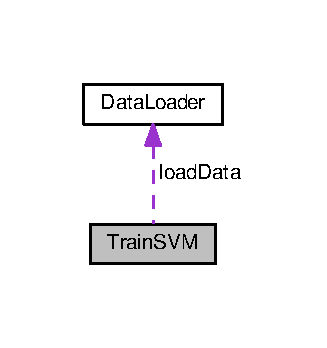
\includegraphics[width=157pt]{classTrainSVM__coll__graph}
\end{center}
\end{figure}
\subsection*{Public Member Functions}
\begin{DoxyCompactItemize}
\item 
\hyperlink{classTrainSVM_a2d30e456094a3eee9aae4aad2023a672}{Train\+S\+VM} ()
\begin{DoxyCompactList}\small\item\em constructor \hyperlink{classTrainSVM}{Train\+S\+VM} \end{DoxyCompactList}\item 
void \hyperlink{classTrainSVM_a4f869e7382bf67edfee56745e3dd46c7}{save\+S\+VM} (std\+::string filename)
\begin{DoxyCompactList}\small\item\em Function to save trained S\+VM. \end{DoxyCompactList}\item 
void \hyperlink{classTrainSVM_aa419880642d9cfb2ef2c094f34971f0b}{start\+Training} ()
\begin{DoxyCompactList}\small\item\em Function to start training. \end{DoxyCompactList}\item 
cv\+::\+Mat \hyperlink{classTrainSVM_a63344677aea94f0e963263619fa5c98f}{prepare\+Data} ()
\begin{DoxyCompactList}\small\item\em Function to change data format into format used by Open\+CV\textquotesingle{}s S\+VM train method. \end{DoxyCompactList}\item 
\hyperlink{classTrainSVM_acd68b7bd056d7497feb97185b6c59f76}{$\sim$\+Train\+S\+VM} ()
\begin{DoxyCompactList}\small\item\em destructor \hyperlink{classTrainSVM}{Train\+S\+VM} \end{DoxyCompactList}\item 
bool \hyperlink{classTrainSVM_a2bd0684e200406c43d3db42e5bda8c52}{directory\+Exist} (const std\+::string \&pathname)
\begin{DoxyCompactList}\small\item\em Function to check existing directory. \end{DoxyCompactList}\item 
void \hyperlink{classTrainSVM_adb7867f2a75e891513ed0c8f95a87642}{set\+Pos\+Directory} (std\+::string dir)
\begin{DoxyCompactList}\small\item\em Function to set directory for positive images. \end{DoxyCompactList}\item 
void \hyperlink{classTrainSVM_ae5eb68ceb9030e0a0cbc13704452f19f}{set\+Neg\+Directory} (std\+::string dir)
\begin{DoxyCompactList}\small\item\em Function to set directory for negative images. \end{DoxyCompactList}\end{DoxyCompactItemize}
\subsection*{Public Attributes}
\begin{DoxyCompactItemize}
\item 
cv\+::\+Ptr$<$ cv\+::ml\+::\+S\+VM $>$ \hyperlink{classTrainSVM_a3b0f3fd57ce484543015573966314368}{svm} = cv\+::ml\+::\+S\+V\+M\+::create()\hypertarget{classTrainSVM_a3b0f3fd57ce484543015573966314368}{}\label{classTrainSVM_a3b0f3fd57ce484543015573966314368}

\begin{DoxyCompactList}\small\item\em Instance to store parameters needed for S\+VM of type cv\+::\+Ptr$<$cv\+::ml\+::\+S\+V\+M$>$ \end{DoxyCompactList}\item 
\hyperlink{classDataLoader}{Data\+Loader} \hyperlink{classTrainSVM_ab12377711608023c25c53efa3fc27b56}{load\+Data}\hypertarget{classTrainSVM_ab12377711608023c25c53efa3fc27b56}{}\label{classTrainSVM_ab12377711608023c25c53efa3fc27b56}

\begin{DoxyCompactList}\small\item\em Instance to take data from class \hyperlink{classDataLoader}{Data\+Loader}. \end{DoxyCompactList}\end{DoxyCompactItemize}


\subsection{Detailed Description}
class \hyperlink{classTrainSVM}{Train\+S\+VM} The class \hyperlink{classTrainSVM}{Train\+S\+VM} trains S\+VM using data from class \hyperlink{classDataLoader}{Data\+Loader} and returns the trained data into a X\+ML file 

\subsection{Constructor \& Destructor Documentation}
\index{Train\+S\+VM@{Train\+S\+VM}!Train\+S\+VM@{Train\+S\+VM}}
\index{Train\+S\+VM@{Train\+S\+VM}!Train\+S\+VM@{Train\+S\+VM}}
\subsubsection[{\texorpdfstring{Train\+S\+V\+M()}{TrainSVM()}}]{\setlength{\rightskip}{0pt plus 5cm}Train\+S\+V\+M\+::\+Train\+S\+VM (
\begin{DoxyParamCaption}
{}
\end{DoxyParamCaption}
)}\hypertarget{classTrainSVM_a2d30e456094a3eee9aae4aad2023a672}{}\label{classTrainSVM_a2d30e456094a3eee9aae4aad2023a672}


constructor \hyperlink{classTrainSVM}{Train\+S\+VM} 


\begin{DoxyParams}{Parameters}
{\em none} & \\
\hline
\end{DoxyParams}
\begin{DoxyReturn}{Returns}
none 
\end{DoxyReturn}
initialising S\+VM model and setting up default values for the parameters

for E\+P\+S\+I\+L\+O\+N\+\_\+\+S\+VR, epsilon in loss function?

From paper, soft classifier \index{Train\+S\+VM@{Train\+S\+VM}!````~Train\+S\+VM@{$\sim$\+Train\+S\+VM}}
\index{````~Train\+S\+VM@{$\sim$\+Train\+S\+VM}!Train\+S\+VM@{Train\+S\+VM}}
\subsubsection[{\texorpdfstring{$\sim$\+Train\+S\+V\+M()}{~TrainSVM()}}]{\setlength{\rightskip}{0pt plus 5cm}Train\+S\+V\+M\+::$\sim$\+Train\+S\+VM (
\begin{DoxyParamCaption}
{}
\end{DoxyParamCaption}
)}\hypertarget{classTrainSVM_acd68b7bd056d7497feb97185b6c59f76}{}\label{classTrainSVM_acd68b7bd056d7497feb97185b6c59f76}


destructor \hyperlink{classTrainSVM}{Train\+S\+VM} 


\begin{DoxyParams}{Parameters}
{\em none} & \\
\hline
\end{DoxyParams}
\begin{DoxyReturn}{Returns}
none 
\end{DoxyReturn}


\subsection{Member Function Documentation}
\index{Train\+S\+VM@{Train\+S\+VM}!directory\+Exist@{directory\+Exist}}
\index{directory\+Exist@{directory\+Exist}!Train\+S\+VM@{Train\+S\+VM}}
\subsubsection[{\texorpdfstring{directory\+Exist(const std\+::string \&pathname)}{directoryExist(const std::string &pathname)}}]{\setlength{\rightskip}{0pt plus 5cm}bool Train\+S\+V\+M\+::directory\+Exist (
\begin{DoxyParamCaption}
\item[{const std\+::string \&}]{pathname}
\end{DoxyParamCaption}
)}\hypertarget{classTrainSVM_a2bd0684e200406c43d3db42e5bda8c52}{}\label{classTrainSVM_a2bd0684e200406c43d3db42e5bda8c52}


Function to check existing directory. 


\begin{DoxyParams}{Parameters}
{\em pathname} & of type string \\
\hline
\end{DoxyParams}
\begin{DoxyReturn}{Returns}
true or false as bool value The following function checks either the file exist or not and returns \textquotesingle{}true\textquotesingle{} if exist and \textquotesingle{}false\textquotesingle{} if not 
\end{DoxyReturn}
\index{Train\+S\+VM@{Train\+S\+VM}!prepare\+Data@{prepare\+Data}}
\index{prepare\+Data@{prepare\+Data}!Train\+S\+VM@{Train\+S\+VM}}
\subsubsection[{\texorpdfstring{prepare\+Data()}{prepareData()}}]{\setlength{\rightskip}{0pt plus 5cm}cv\+::\+Mat Train\+S\+V\+M\+::prepare\+Data (
\begin{DoxyParamCaption}
{}
\end{DoxyParamCaption}
)}\hypertarget{classTrainSVM_a63344677aea94f0e963263619fa5c98f}{}\label{classTrainSVM_a63344677aea94f0e963263619fa5c98f}


Function to change data format into format used by Open\+CV\textquotesingle{}s S\+VM train method. 


\begin{DoxyParams}{Parameters}
{\em filename} & of type string \\
\hline
\end{DoxyParams}
\begin{DoxyReturn}{Returns}
training data of type cv\+::\+Mat 
\end{DoxyReturn}
temp is used to store data values in the format as required to train the S\+VM model \index{Train\+S\+VM@{Train\+S\+VM}!save\+S\+VM@{save\+S\+VM}}
\index{save\+S\+VM@{save\+S\+VM}!Train\+S\+VM@{Train\+S\+VM}}
\subsubsection[{\texorpdfstring{save\+S\+V\+M(std\+::string filename)}{saveSVM(std::string filename)}}]{\setlength{\rightskip}{0pt plus 5cm}void Train\+S\+V\+M\+::save\+S\+VM (
\begin{DoxyParamCaption}
\item[{std\+::string}]{filename}
\end{DoxyParamCaption}
)}\hypertarget{classTrainSVM_a4f869e7382bf67edfee56745e3dd46c7}{}\label{classTrainSVM_a4f869e7382bf67edfee56745e3dd46c7}


Function to save trained S\+VM. 


\begin{DoxyParams}{Parameters}
{\em filename} & of type string \\
\hline
\end{DoxyParams}
\begin{DoxyReturn}{Returns}
none The following function saves trained S\+VM in a file and takes the filename 
\end{DoxyReturn}
\index{Train\+S\+VM@{Train\+S\+VM}!set\+Neg\+Directory@{set\+Neg\+Directory}}
\index{set\+Neg\+Directory@{set\+Neg\+Directory}!Train\+S\+VM@{Train\+S\+VM}}
\subsubsection[{\texorpdfstring{set\+Neg\+Directory(std\+::string dir)}{setNegDirectory(std::string dir)}}]{\setlength{\rightskip}{0pt plus 5cm}void Train\+S\+V\+M\+::set\+Neg\+Directory (
\begin{DoxyParamCaption}
\item[{std\+::string}]{dir}
\end{DoxyParamCaption}
)}\hypertarget{classTrainSVM_ae5eb68ceb9030e0a0cbc13704452f19f}{}\label{classTrainSVM_ae5eb68ceb9030e0a0cbc13704452f19f}


Function to set directory for negative images. 


\begin{DoxyParams}{Parameters}
{\em dir} & of type string \\
\hline
\end{DoxyParams}
\begin{DoxyReturn}{Returns}
none The following function saves the negative images in a directory 
\end{DoxyReturn}
\index{Train\+S\+VM@{Train\+S\+VM}!set\+Pos\+Directory@{set\+Pos\+Directory}}
\index{set\+Pos\+Directory@{set\+Pos\+Directory}!Train\+S\+VM@{Train\+S\+VM}}
\subsubsection[{\texorpdfstring{set\+Pos\+Directory(std\+::string dir)}{setPosDirectory(std::string dir)}}]{\setlength{\rightskip}{0pt plus 5cm}void Train\+S\+V\+M\+::set\+Pos\+Directory (
\begin{DoxyParamCaption}
\item[{std\+::string}]{dir}
\end{DoxyParamCaption}
)}\hypertarget{classTrainSVM_adb7867f2a75e891513ed0c8f95a87642}{}\label{classTrainSVM_adb7867f2a75e891513ed0c8f95a87642}


Function to set directory for positive images. 


\begin{DoxyParams}{Parameters}
{\em dir} & of type string \\
\hline
\end{DoxyParams}
\begin{DoxyReturn}{Returns}
none The following function saves the positive images in a directory 
\end{DoxyReturn}
\index{Train\+S\+VM@{Train\+S\+VM}!start\+Training@{start\+Training}}
\index{start\+Training@{start\+Training}!Train\+S\+VM@{Train\+S\+VM}}
\subsubsection[{\texorpdfstring{start\+Training()}{startTraining()}}]{\setlength{\rightskip}{0pt plus 5cm}void Train\+S\+V\+M\+::start\+Training (
\begin{DoxyParamCaption}
{}
\end{DoxyParamCaption}
)}\hypertarget{classTrainSVM_aa419880642d9cfb2ef2c094f34971f0b}{}\label{classTrainSVM_aa419880642d9cfb2ef2c094f34971f0b}


Function to start training. 


\begin{DoxyParams}{Parameters}
{\em none} & \\
\hline
\end{DoxyParams}
\begin{DoxyReturn}{Returns}
none The following function initiates S\+VM training 
\end{DoxyReturn}


The documentation for this class was generated from the following files\+:\begin{DoxyCompactItemize}
\item 
include/\hyperlink{TrainSVM_8hpp}{Train\+S\+V\+M.\+hpp}\item 
app/\hyperlink{TrainSVM_8cpp}{Train\+S\+V\+M.\+cpp}\end{DoxyCompactItemize}

\hypertarget{classVisionInput}{}\section{Vision\+Input Class Reference}
\label{classVisionInput}\index{Vision\+Input@{Vision\+Input}}


class \hyperlink{classVisionInput}{Vision\+Input} The class \hyperlink{classVisionInput}{Vision\+Input} gives different functionalities to use H\+OG feature based Human detection, so that it can be used with live videos from camera sensor or saved videos and image files.  




{\ttfamily \#include $<$Vision\+Input.\+hpp$>$}



Collaboration diagram for Vision\+Input\+:
\nopagebreak
\begin{figure}[H]
\begin{center}
\leavevmode
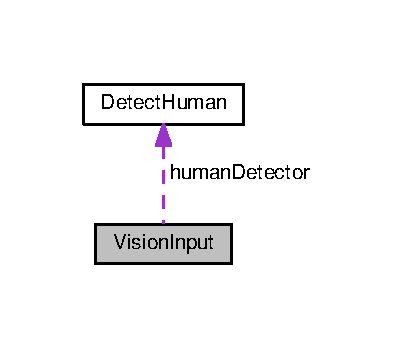
\includegraphics[width=189pt]{classVisionInput__coll__graph}
\end{center}
\end{figure}
\subsection*{Public Member Functions}
\begin{DoxyCompactItemize}
\item 
\hyperlink{classVisionInput_aaea2418176f6766cfd7ae09f333d176a}{Vision\+Input} ()
\begin{DoxyCompactList}\small\item\em constructor \hyperlink{classVisionInput}{Vision\+Input} \end{DoxyCompactList}\item 
void \hyperlink{classVisionInput_a54caed2ca4579dbbf274b2730bf11a01}{detect\+With\+Camera} (int camera\+Code)
\begin{DoxyCompactList}\small\item\em This method starts human detection from specified camera feed. \end{DoxyCompactList}\item 
void \hyperlink{classVisionInput_a37b18210c09b26d1fb0cddf930882857}{detect\+With\+Video\+File} (std\+::string filename)
\begin{DoxyCompactList}\small\item\em This method starts human detection from specified video file. \end{DoxyCompactList}\item 
void \hyperlink{classVisionInput_a6e00b038651a43978a351c3a54d27005}{detect\+With\+Image} (std\+::string filename)
\begin{DoxyCompactList}\small\item\em This method starts human detection from specified image file. \end{DoxyCompactList}\item 
void \hyperlink{classVisionInput_ad7e80a1b7ee9f63cb56ee0b6a1e96351}{setup\+Detector} (std\+::string S\+V\+M\+Filename)
\begin{DoxyCompactList}\small\item\em This method sets which S\+VM model will be used for detection. \end{DoxyCompactList}\item 
void \hyperlink{classVisionInput_ac76ded14c04baccb34d8cc3277258f68}{show\+Image\+With\+Box} ()
\begin{DoxyCompactList}\small\item\em This method creates bounding boxes around detected humans. \end{DoxyCompactList}\item 
\hyperlink{classVisionInput_ab7800dddb115d9ba6da676b496b03259}{$\sim$\+Vision\+Input} ()
\begin{DoxyCompactList}\small\item\em destructor \hyperlink{classVisionInput}{Vision\+Input} \end{DoxyCompactList}\end{DoxyCompactItemize}
\subsection*{Public Attributes}
\begin{DoxyCompactItemize}
\item 
cv\+::\+Mat \hyperlink{classVisionInput_a70fb6d723dd13355981e263f11b798ab}{image}\hypertarget{classVisionInput_a70fb6d723dd13355981e263f11b798ab}{}\label{classVisionInput_a70fb6d723dd13355981e263f11b798ab}

\begin{DoxyCompactList}\small\item\em Container to store an image. \end{DoxyCompactList}\item 
\hyperlink{classDetectHuman}{Detect\+Human} \hyperlink{classVisionInput_a9888dff84fef69e454dbd2a38735d2da}{human\+Detector}\hypertarget{classVisionInput_a9888dff84fef69e454dbd2a38735d2da}{}\label{classVisionInput_a9888dff84fef69e454dbd2a38735d2da}

\begin{DoxyCompactList}\small\item\em Instance created of Detec\+Human class for human detection with data fedd. \end{DoxyCompactList}\item 
std\+::vector$<$ cv\+::\+Rect $>$ \hyperlink{classVisionInput_af46eecf1faba0b375ce0acbbc4605043}{bounding\+Boxes}\hypertarget{classVisionInput_af46eecf1faba0b375ce0acbbc4605043}{}\label{classVisionInput_af46eecf1faba0b375ce0acbbc4605043}

\begin{DoxyCompactList}\small\item\em Container to store detected human positions in form of pixel coordinates. \end{DoxyCompactList}\end{DoxyCompactItemize}


\subsection{Detailed Description}
class \hyperlink{classVisionInput}{Vision\+Input} The class \hyperlink{classVisionInput}{Vision\+Input} gives different functionalities to use H\+OG feature based Human detection, so that it can be used with live videos from camera sensor or saved videos and image files. 

\subsection{Constructor \& Destructor Documentation}
\index{Vision\+Input@{Vision\+Input}!Vision\+Input@{Vision\+Input}}
\index{Vision\+Input@{Vision\+Input}!Vision\+Input@{Vision\+Input}}
\subsubsection[{\texorpdfstring{Vision\+Input()}{VisionInput()}}]{\setlength{\rightskip}{0pt plus 5cm}Vision\+Input\+::\+Vision\+Input (
\begin{DoxyParamCaption}
{}
\end{DoxyParamCaption}
)}\hypertarget{classVisionInput_aaea2418176f6766cfd7ae09f333d176a}{}\label{classVisionInput_aaea2418176f6766cfd7ae09f333d176a}


constructor \hyperlink{classVisionInput}{Vision\+Input} 


\begin{DoxyParams}{Parameters}
{\em none} & \\
\hline
\end{DoxyParams}
\begin{DoxyReturn}{Returns}
none 
\end{DoxyReturn}
\index{Vision\+Input@{Vision\+Input}!````~Vision\+Input@{$\sim$\+Vision\+Input}}
\index{````~Vision\+Input@{$\sim$\+Vision\+Input}!Vision\+Input@{Vision\+Input}}
\subsubsection[{\texorpdfstring{$\sim$\+Vision\+Input()}{~VisionInput()}}]{\setlength{\rightskip}{0pt plus 5cm}Vision\+Input\+::$\sim$\+Vision\+Input (
\begin{DoxyParamCaption}
{}
\end{DoxyParamCaption}
)}\hypertarget{classVisionInput_ab7800dddb115d9ba6da676b496b03259}{}\label{classVisionInput_ab7800dddb115d9ba6da676b496b03259}


destructor \hyperlink{classVisionInput}{Vision\+Input} 


\begin{DoxyParams}{Parameters}
{\em none} & \\
\hline
\end{DoxyParams}
\begin{DoxyReturn}{Returns}
none 
\end{DoxyReturn}


\subsection{Member Function Documentation}
\index{Vision\+Input@{Vision\+Input}!detect\+With\+Camera@{detect\+With\+Camera}}
\index{detect\+With\+Camera@{detect\+With\+Camera}!Vision\+Input@{Vision\+Input}}
\subsubsection[{\texorpdfstring{detect\+With\+Camera(int camera\+Code)}{detectWithCamera(int cameraCode)}}]{\setlength{\rightskip}{0pt plus 5cm}void Vision\+Input\+::detect\+With\+Camera (
\begin{DoxyParamCaption}
\item[{int}]{camera\+Code}
\end{DoxyParamCaption}
)}\hypertarget{classVisionInput_a54caed2ca4579dbbf274b2730bf11a01}{}\label{classVisionInput_a54caed2ca4579dbbf274b2730bf11a01}


This method starts human detection from specified camera feed. 


\begin{DoxyParams}{Parameters}
{\em camera\+Code} & of type int \\
\hline
\end{DoxyParams}
\begin{DoxyReturn}{Returns}
none  Camera code depends which camera you want to use. Normally code 0 is used to start reading data from webcam. 
\end{DoxyReturn}
Setting up Camera object

Finding humans

Display image with bounding around humans

Press E\+SC to exit \index{Vision\+Input@{Vision\+Input}!detect\+With\+Image@{detect\+With\+Image}}
\index{detect\+With\+Image@{detect\+With\+Image}!Vision\+Input@{Vision\+Input}}
\subsubsection[{\texorpdfstring{detect\+With\+Image(std\+::string filename)}{detectWithImage(std::string filename)}}]{\setlength{\rightskip}{0pt plus 5cm}void Vision\+Input\+::detect\+With\+Image (
\begin{DoxyParamCaption}
\item[{std\+::string}]{filename}
\end{DoxyParamCaption}
)}\hypertarget{classVisionInput_a6e00b038651a43978a351c3a54d27005}{}\label{classVisionInput_a6e00b038651a43978a351c3a54d27005}


This method starts human detection from specified image file. 


\begin{DoxyParams}{Parameters}
{\em camera\+Code} & of type string \\
\hline
\end{DoxyParams}
\begin{DoxyReturn}{Returns}
none  Provide an image filename with full path in order to run human detection with image files 
\end{DoxyReturn}
\index{Vision\+Input@{Vision\+Input}!detect\+With\+Video\+File@{detect\+With\+Video\+File}}
\index{detect\+With\+Video\+File@{detect\+With\+Video\+File}!Vision\+Input@{Vision\+Input}}
\subsubsection[{\texorpdfstring{detect\+With\+Video\+File(std\+::string filename)}{detectWithVideoFile(std::string filename)}}]{\setlength{\rightskip}{0pt plus 5cm}void Vision\+Input\+::detect\+With\+Video\+File (
\begin{DoxyParamCaption}
\item[{std\+::string}]{filename}
\end{DoxyParamCaption}
)}\hypertarget{classVisionInput_a37b18210c09b26d1fb0cddf930882857}{}\label{classVisionInput_a37b18210c09b26d1fb0cddf930882857}


This method starts human detection from specified video file. 


\begin{DoxyParams}{Parameters}
{\em filename} & of type string \\
\hline
\end{DoxyParams}
\begin{DoxyReturn}{Returns}
none  Provide a video filename with full path in order to run human detection with videofiles 
\end{DoxyReturn}
\index{Vision\+Input@{Vision\+Input}!setup\+Detector@{setup\+Detector}}
\index{setup\+Detector@{setup\+Detector}!Vision\+Input@{Vision\+Input}}
\subsubsection[{\texorpdfstring{setup\+Detector(std\+::string S\+V\+M\+Filename)}{setupDetector(std::string SVMFilename)}}]{\setlength{\rightskip}{0pt plus 5cm}void Vision\+Input\+::setup\+Detector (
\begin{DoxyParamCaption}
\item[{std\+::string}]{S\+V\+M\+Filename}
\end{DoxyParamCaption}
)}\hypertarget{classVisionInput_ad7e80a1b7ee9f63cb56ee0b6a1e96351}{}\label{classVisionInput_ad7e80a1b7ee9f63cb56ee0b6a1e96351}


This method sets which S\+VM model will be used for detection. 


\begin{DoxyParams}{Parameters}
{\em S\+V\+M\+Filename} & of type string \\
\hline
\end{DoxyParams}
\begin{DoxyReturn}{Returns}
none  You can provide your own S\+VM classifier or you can use default classifier provided with Open\+CV 
\end{DoxyReturn}
Check if file already exist or not \index{Vision\+Input@{Vision\+Input}!show\+Image\+With\+Box@{show\+Image\+With\+Box}}
\index{show\+Image\+With\+Box@{show\+Image\+With\+Box}!Vision\+Input@{Vision\+Input}}
\subsubsection[{\texorpdfstring{show\+Image\+With\+Box()}{showImageWithBox()}}]{\setlength{\rightskip}{0pt plus 5cm}void Vision\+Input\+::show\+Image\+With\+Box (
\begin{DoxyParamCaption}
{}
\end{DoxyParamCaption}
)}\hypertarget{classVisionInput_ac76ded14c04baccb34d8cc3277258f68}{}\label{classVisionInput_ac76ded14c04baccb34d8cc3277258f68}


This method creates bounding boxes around detected humans. 


\begin{DoxyParams}{Parameters}
{\em none} & \\
\hline
\end{DoxyParams}
\begin{DoxyReturn}{Returns}
none 
\end{DoxyReturn}
Dimensions of bounding box

cv\+::imshow(\char`\"{}\+A\+C\+M\+E Robotics\char`\"{}, image); 

The documentation for this class was generated from the following files\+:\begin{DoxyCompactItemize}
\item 
include/\hyperlink{VisionInput_8hpp}{Vision\+Input.\+hpp}\item 
app/\hyperlink{VisionInput_8cpp}{Vision\+Input.\+cpp}\end{DoxyCompactItemize}

\chapter{File Documentation}
\hypertarget{DataLoader_8cpp}{}\section{app/\+Data\+Loader.cpp File Reference}
\label{DataLoader_8cpp}\index{app/\+Data\+Loader.\+cpp@{app/\+Data\+Loader.\+cpp}}


\hyperlink{classDataLoader}{Data\+Loader} method implementation.  


{\ttfamily \#include $<$Data\+Loader.\+hpp$>$}\\*
Include dependency graph for Data\+Loader.\+cpp\+:
\nopagebreak
\begin{figure}[H]
\begin{center}
\leavevmode
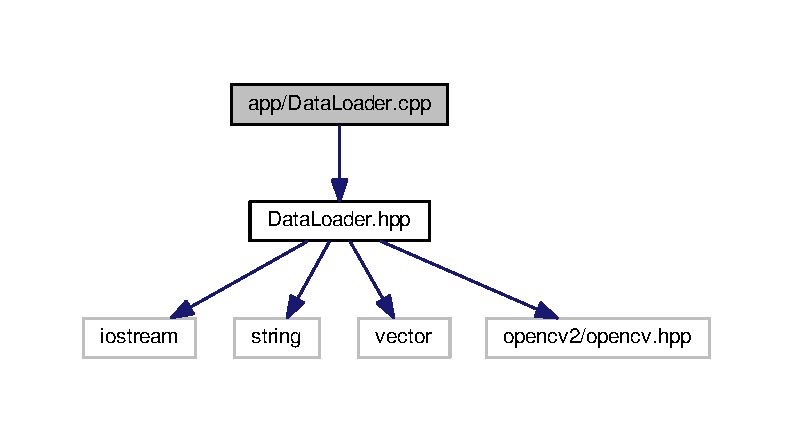
\includegraphics[width=350pt]{DataLoader_8cpp__incl}
\end{center}
\end{figure}


\subsection{Detailed Description}
\hyperlink{classDataLoader}{Data\+Loader} method implementation. 

\begin{DoxyAuthor}{Author}
Aman Virmani (Aman\+Virmani) Driver 

Naman Gupta (namangupta98) Navigator 

Saumil Shah (Saumil\+Shah66) Design Keeper 
\end{DoxyAuthor}
\begin{DoxyCopyright}{Copyright}
M\+IT License 
\end{DoxyCopyright}

\hypertarget{DetectHuman_8cpp}{}\section{app/\+Detect\+Human.cpp File Reference}
\label{DetectHuman_8cpp}\index{app/\+Detect\+Human.\+cpp@{app/\+Detect\+Human.\+cpp}}


\hyperlink{classDetectHuman}{Detect\+Human} Class declaration  Implementation of class methods to detect humans using an S\+VM model trained on H\+OG features.  


{\ttfamily \#include $<$Detect\+Human.\+hpp$>$}\\*
Include dependency graph for Detect\+Human.\+cpp\+:
\nopagebreak
\begin{figure}[H]
\begin{center}
\leavevmode
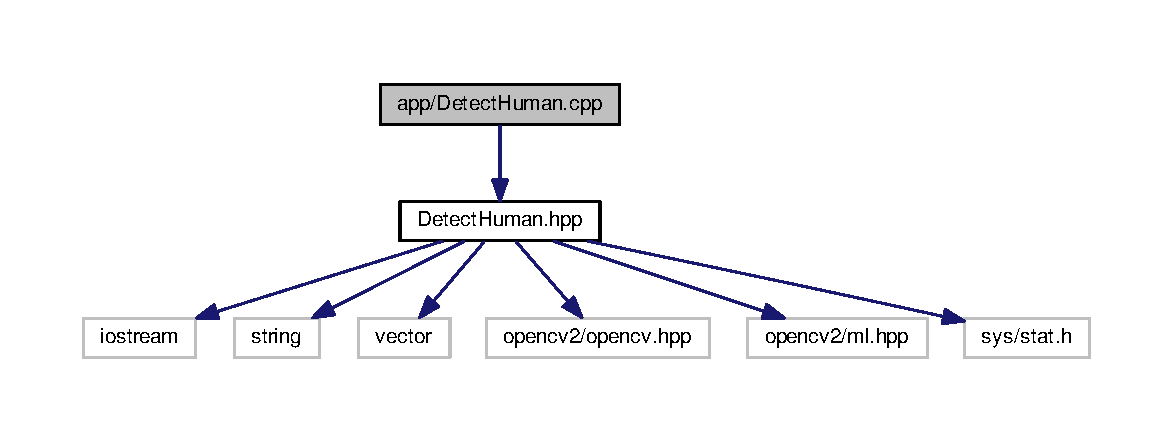
\includegraphics[width=350pt]{DetectHuman_8cpp__incl}
\end{center}
\end{figure}


\subsection{Detailed Description}
\hyperlink{classDetectHuman}{Detect\+Human} Class declaration  Implementation of class methods to detect humans using an S\+VM model trained on H\+OG features. 

\begin{DoxyAuthor}{Author}
Naman Gupta (namangupta98) Driver 

Saumil Shah (Saumil\+Shah66) Design Keeper 

Aman Virmani (Aman\+Virmani) Navigator 
\end{DoxyAuthor}
\begin{DoxyCopyright}{Copyright}
M\+IT License 
\end{DoxyCopyright}

\hypertarget{TrainSVM_8cpp}{}\section{app/\+Train\+S\+VM.cpp File Reference}
\label{TrainSVM_8cpp}\index{app/\+Train\+S\+V\+M.\+cpp@{app/\+Train\+S\+V\+M.\+cpp}}


\hyperlink{classTrainSVM}{Train\+S\+VM} Class declaration  Implementation of class methods to train S\+VM using data from class \hyperlink{classDataLoader}{Data\+Loader}.  


{\ttfamily \#include $<$Train\+S\+V\+M.\+hpp$>$}\\*
Include dependency graph for Train\+S\+V\+M.\+cpp\+:
\nopagebreak
\begin{figure}[H]
\begin{center}
\leavevmode
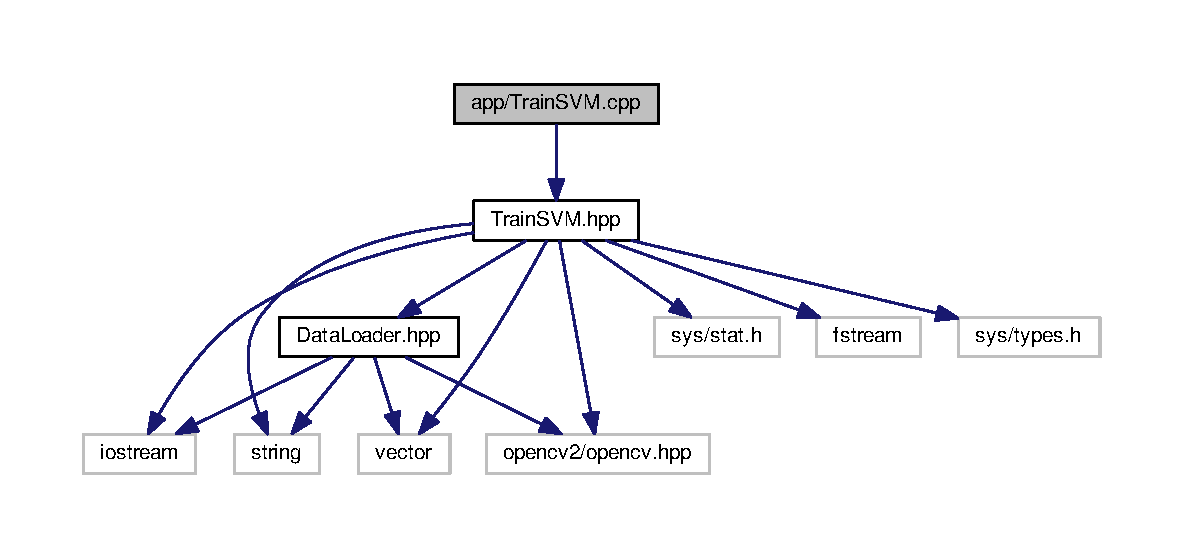
\includegraphics[width=350pt]{TrainSVM_8cpp__incl}
\end{center}
\end{figure}


\subsection{Detailed Description}
\hyperlink{classTrainSVM}{Train\+S\+VM} Class declaration  Implementation of class methods to train S\+VM using data from class \hyperlink{classDataLoader}{Data\+Loader}. 

\begin{DoxyAuthor}{Author}
Aman Virmani (Aman\+Virmani) Driver 

Naman Gupta (namangupta98) Navigator 

Saumil Shah (Saumil\+Shah66) Design Keeper 
\end{DoxyAuthor}
\begin{DoxyCopyright}{Copyright}
M\+IT License 
\end{DoxyCopyright}

\hypertarget{VisionInput_8cpp}{}\section{app/\+Vision\+Input.cpp File Reference}
\label{VisionInput_8cpp}\index{app/\+Vision\+Input.\+cpp@{app/\+Vision\+Input.\+cpp}}


\hyperlink{classVisionInput}{Vision\+Input} Class declaration  Implementation of class methods to train S\+VM using data from class \hyperlink{classDataLoader}{Data\+Loader}.  


{\ttfamily \#include $<$Vision\+Input.\+hpp$>$}\\*
Include dependency graph for Vision\+Input.\+cpp\+:
\nopagebreak
\begin{figure}[H]
\begin{center}
\leavevmode
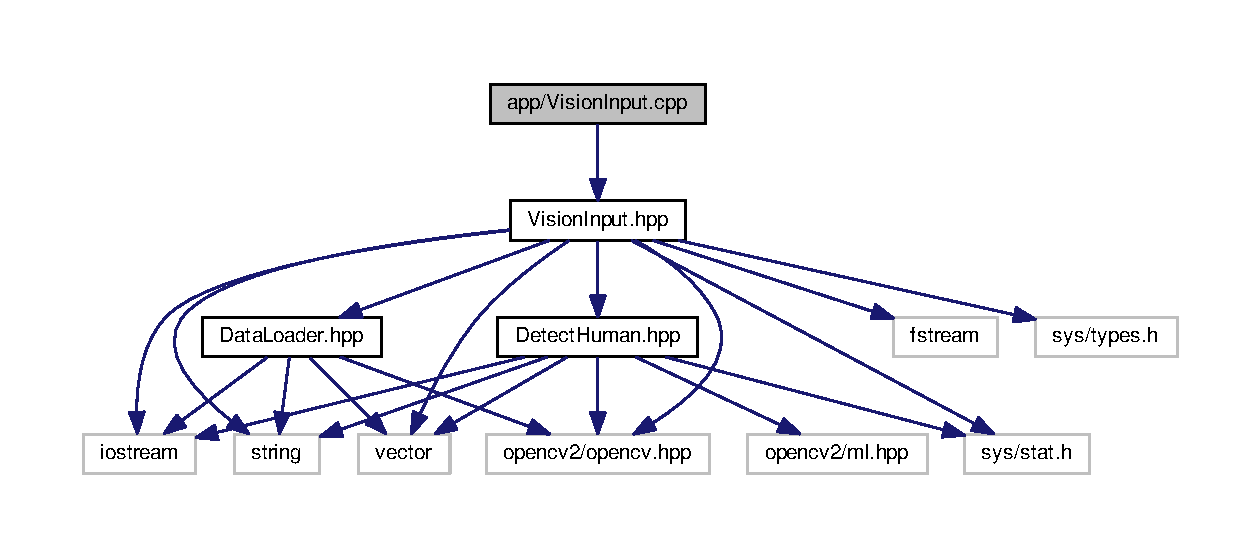
\includegraphics[width=350pt]{VisionInput_8cpp__incl}
\end{center}
\end{figure}


\subsection{Detailed Description}
\hyperlink{classVisionInput}{Vision\+Input} Class declaration  Implementation of class methods to train S\+VM using data from class \hyperlink{classDataLoader}{Data\+Loader}. 

\begin{DoxyAuthor}{Author}
Naman Gupta (namangupta98) Driver 

Saumil Shah (Saumil\+Shah66) Design Keeper 

Aman Virmani (Aman\+Virmani) Navigator 
\end{DoxyAuthor}
\begin{DoxyCopyright}{Copyright}
M\+IT License 
\end{DoxyCopyright}

\hypertarget{DataLoader_8hpp}{}\section{include/\+Data\+Loader.hpp File Reference}
\label{DataLoader_8hpp}\index{include/\+Data\+Loader.\+hpp@{include/\+Data\+Loader.\+hpp}}


\hyperlink{classDataLoader}{Data\+Loader} Class declaration  Declared functions Class to read data from files.  


{\ttfamily \#include $<$iostream$>$}\\*
{\ttfamily \#include $<$string$>$}\\*
{\ttfamily \#include $<$vector$>$}\\*
{\ttfamily \#include $<$opencv2/opencv.\+hpp$>$}\\*
Include dependency graph for Data\+Loader.\+hpp\+:
\nopagebreak
\begin{figure}[H]
\begin{center}
\leavevmode
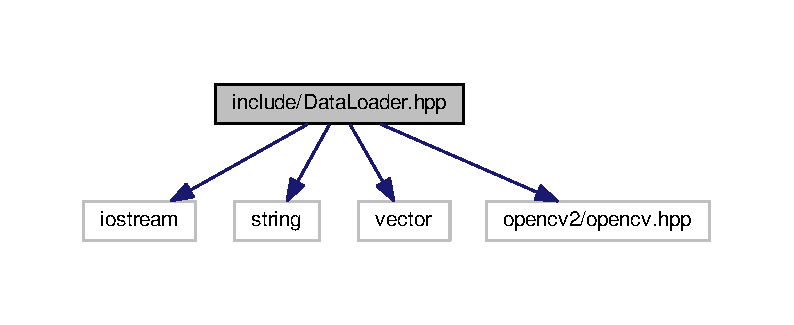
\includegraphics[width=350pt]{DataLoader_8hpp__incl}
\end{center}
\end{figure}
This graph shows which files directly or indirectly include this file\+:
\nopagebreak
\begin{figure}[H]
\begin{center}
\leavevmode
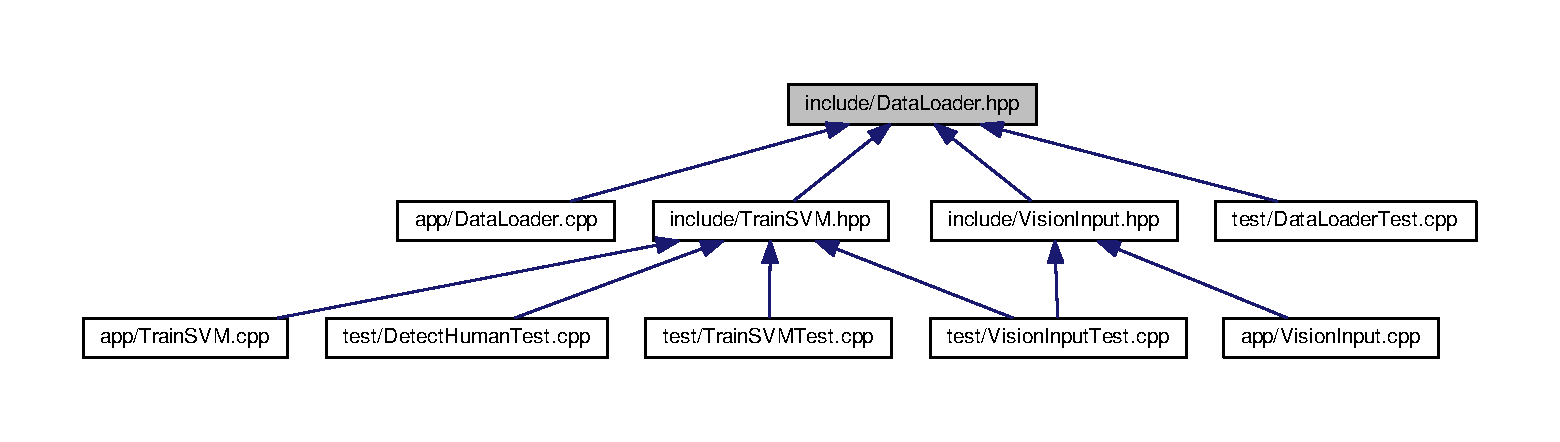
\includegraphics[width=350pt]{DataLoader_8hpp__dep__incl}
\end{center}
\end{figure}
\subsection*{Classes}
\begin{DoxyCompactItemize}
\item 
class \hyperlink{classDataLoader}{Data\+Loader}
\begin{DoxyCompactList}\small\item\em class \hyperlink{classDataLoader}{Data\+Loader} The class \hyperlink{classDataLoader}{Data\+Loader} reads data from files for training purposes and creates H\+OG feature for every image. \end{DoxyCompactList}\end{DoxyCompactItemize}


\subsection{Detailed Description}
\hyperlink{classDataLoader}{Data\+Loader} Class declaration  Declared functions Class to read data from files. 

\begin{DoxyAuthor}{Author}
Saumil Shah (Saumil\+Shah66) Driver 

Naman Gupta (namangupta98) Navigator 

Aman Virmani (Aman\+Virmani) Design Keeper 
\end{DoxyAuthor}
\begin{DoxyCopyright}{Copyright}
M\+IT License 
\end{DoxyCopyright}

\hypertarget{DetectHuman_8hpp}{}\section{include/\+Detect\+Human.hpp File Reference}
\label{DetectHuman_8hpp}\index{include/\+Detect\+Human.\+hpp@{include/\+Detect\+Human.\+hpp}}


\hyperlink{classDetectHuman}{Detect\+Human} Class declaration  Declared functions Class to detect humans using an S\+VM model trained on H\+OG features.  


{\ttfamily \#include $<$iostream$>$}\\*
{\ttfamily \#include $<$string$>$}\\*
{\ttfamily \#include $<$vector$>$}\\*
{\ttfamily \#include $<$opencv2/opencv.\+hpp$>$}\\*
{\ttfamily \#include $<$opencv2/ml.\+hpp$>$}\\*
{\ttfamily \#include $<$sys/stat.\+h$>$}\\*
Include dependency graph for Detect\+Human.\+hpp\+:
\nopagebreak
\begin{figure}[H]
\begin{center}
\leavevmode
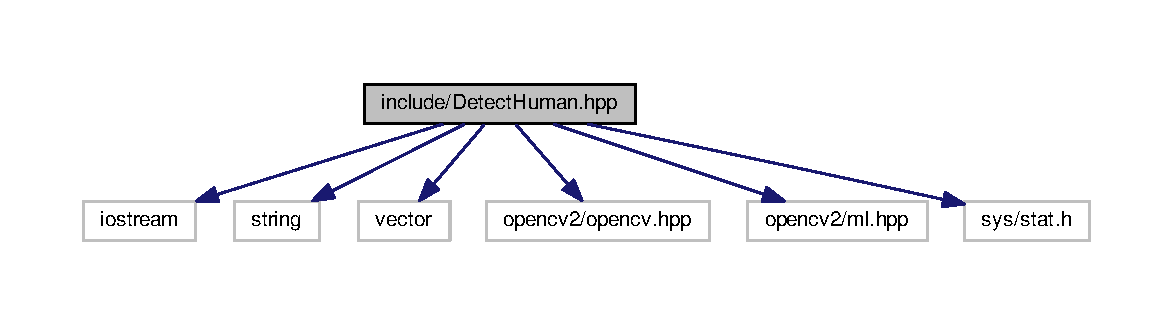
\includegraphics[width=350pt]{DetectHuman_8hpp__incl}
\end{center}
\end{figure}
This graph shows which files directly or indirectly include this file\+:
\nopagebreak
\begin{figure}[H]
\begin{center}
\leavevmode
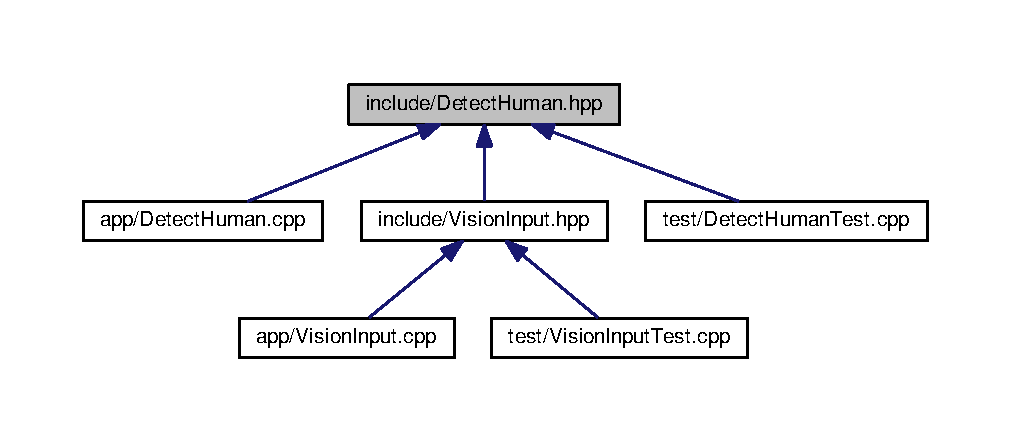
\includegraphics[width=350pt]{DetectHuman_8hpp__dep__incl}
\end{center}
\end{figure}
\subsection*{Classes}
\begin{DoxyCompactItemize}
\item 
class \hyperlink{classDetectHuman}{Detect\+Human}
\begin{DoxyCompactList}\small\item\em class \hyperlink{classDetectHuman}{Detect\+Human} The class \hyperlink{classDetectHuman}{Detect\+Human} uses a trained S\+VM model to detect humans in an image and returns the pixel coordinates of the bounding boxes containing humans in an image \end{DoxyCompactList}\end{DoxyCompactItemize}


\subsection{Detailed Description}
\hyperlink{classDetectHuman}{Detect\+Human} Class declaration  Declared functions Class to detect humans using an S\+VM model trained on H\+OG features. 

\begin{DoxyAuthor}{Author}
Saumil Shah (Saumil\+Shah66) Driver 

Naman Gupta (namangupta98) Navigator 

Aman Virmani (Aman\+Virmani) Design Keeper 
\end{DoxyAuthor}
\begin{DoxyCopyright}{Copyright}
M\+IT License 
\end{DoxyCopyright}

\hypertarget{TrainSVM_8hpp}{}\section{include/\+Train\+S\+VM.hpp File Reference}
\label{TrainSVM_8hpp}\index{include/\+Train\+S\+V\+M.\+hpp@{include/\+Train\+S\+V\+M.\+hpp}}


\hyperlink{classTrainSVM}{Train\+S\+VM} Class declaration  Declared functions Class to train S\+VM using data from class \hyperlink{classDataLoader}{Data\+Loader}.  


{\ttfamily \#include $<$iostream$>$}\\*
{\ttfamily \#include $<$string$>$}\\*
{\ttfamily \#include $<$vector$>$}\\*
{\ttfamily \#include $<$opencv2/opencv.\+hpp$>$}\\*
{\ttfamily \#include $<$Data\+Loader.\+hpp$>$}\\*
{\ttfamily \#include $<$sys/stat.\+h$>$}\\*
{\ttfamily \#include $<$fstream$>$}\\*
{\ttfamily \#include $<$sys/types.\+h$>$}\\*
Include dependency graph for Train\+S\+V\+M.\+hpp\+:
\nopagebreak
\begin{figure}[H]
\begin{center}
\leavevmode
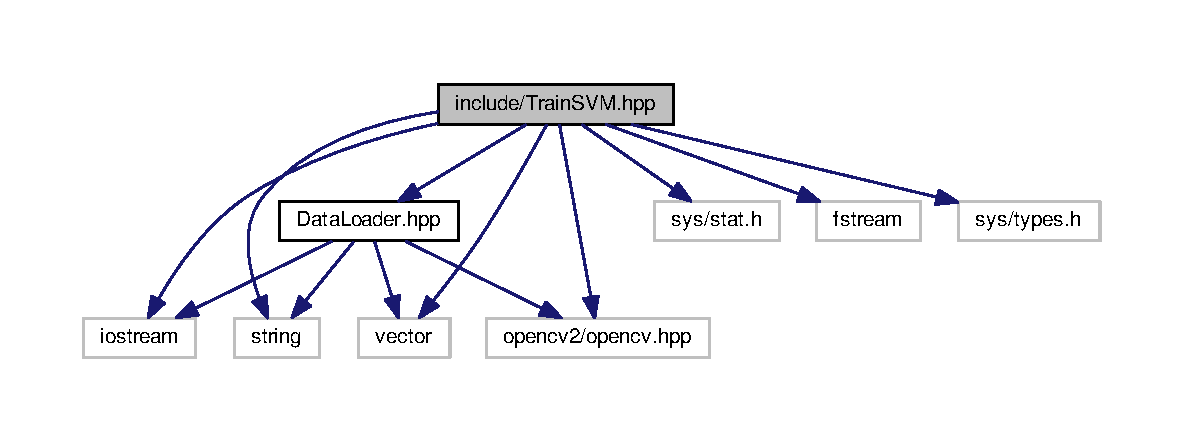
\includegraphics[width=350pt]{TrainSVM_8hpp__incl}
\end{center}
\end{figure}
This graph shows which files directly or indirectly include this file\+:
\nopagebreak
\begin{figure}[H]
\begin{center}
\leavevmode
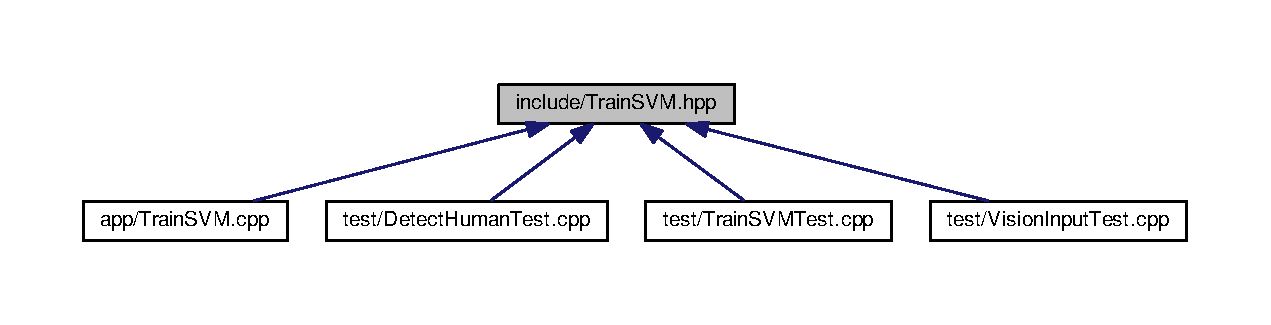
\includegraphics[width=350pt]{TrainSVM_8hpp__dep__incl}
\end{center}
\end{figure}
\subsection*{Classes}
\begin{DoxyCompactItemize}
\item 
class \hyperlink{classTrainSVM}{Train\+S\+VM}
\begin{DoxyCompactList}\small\item\em class \hyperlink{classTrainSVM}{Train\+S\+VM} The class \hyperlink{classTrainSVM}{Train\+S\+VM} trains S\+VM using data from class \hyperlink{classDataLoader}{Data\+Loader} and returns the trained data into a X\+ML file \end{DoxyCompactList}\end{DoxyCompactItemize}


\subsection{Detailed Description}
\hyperlink{classTrainSVM}{Train\+S\+VM} Class declaration  Declared functions Class to train S\+VM using data from class \hyperlink{classDataLoader}{Data\+Loader}. 

\begin{DoxyAuthor}{Author}
Saumil Shah (Saumil\+Shah66) Driver 

Naman Gupta (namangupta98) Navigator 

Aman Virmani (Aman\+Virmani) Design Keeper 
\end{DoxyAuthor}
\begin{DoxyCopyright}{Copyright}
M\+IT License 
\end{DoxyCopyright}

\hypertarget{VisionInput_8hpp}{}\section{include/\+Vision\+Input.hpp File Reference}
\label{VisionInput_8hpp}\index{include/\+Vision\+Input.\+hpp@{include/\+Vision\+Input.\+hpp}}


\hyperlink{classVisionInput}{Vision\+Input} Class declaration  Declared functions Class to get data for realtime detection.  


{\ttfamily \#include $<$iostream$>$}\\*
{\ttfamily \#include $<$string$>$}\\*
{\ttfamily \#include $<$vector$>$}\\*
{\ttfamily \#include $<$opencv2/opencv.\+hpp$>$}\\*
{\ttfamily \#include $<$Data\+Loader.\+hpp$>$}\\*
{\ttfamily \#include $<$sys/stat.\+h$>$}\\*
{\ttfamily \#include $<$fstream$>$}\\*
{\ttfamily \#include $<$sys/types.\+h$>$}\\*
{\ttfamily \#include $<$Detect\+Human.\+hpp$>$}\\*
Include dependency graph for Vision\+Input.\+hpp\+:
\nopagebreak
\begin{figure}[H]
\begin{center}
\leavevmode
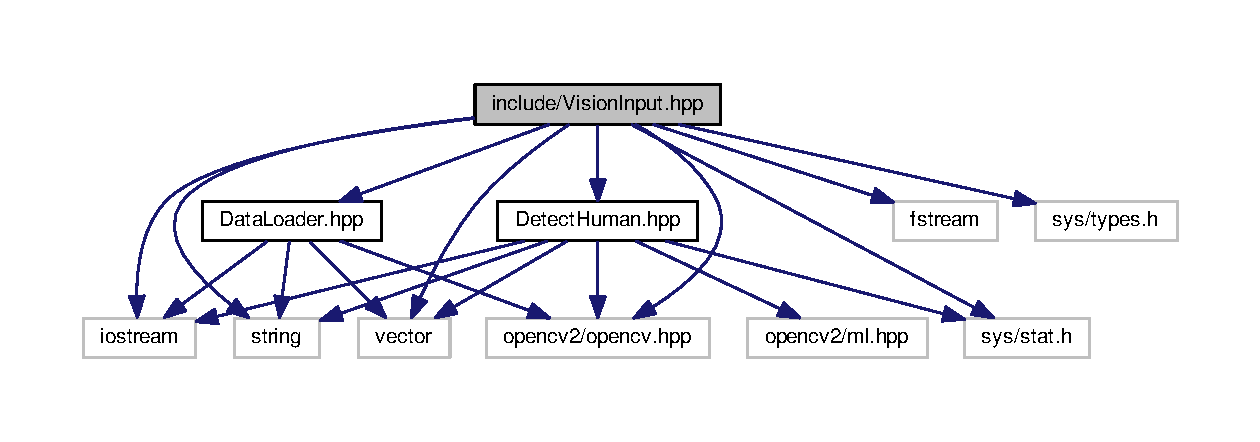
\includegraphics[width=350pt]{VisionInput_8hpp__incl}
\end{center}
\end{figure}
This graph shows which files directly or indirectly include this file\+:
\nopagebreak
\begin{figure}[H]
\begin{center}
\leavevmode
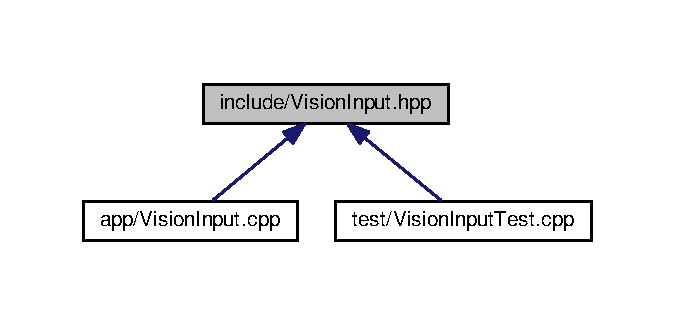
\includegraphics[width=324pt]{VisionInput_8hpp__dep__incl}
\end{center}
\end{figure}
\subsection*{Classes}
\begin{DoxyCompactItemize}
\item 
class \hyperlink{classVisionInput}{Vision\+Input}
\begin{DoxyCompactList}\small\item\em class \hyperlink{classVisionInput}{Vision\+Input} The class \hyperlink{classVisionInput}{Vision\+Input} gives different functionalities to use H\+OG feature based Human detection, so that it can be used with live videos from camera sensor or saved videos and image files. \end{DoxyCompactList}\end{DoxyCompactItemize}


\subsection{Detailed Description}
\hyperlink{classVisionInput}{Vision\+Input} Class declaration  Declared functions Class to get data for realtime detection. 

\begin{DoxyAuthor}{Author}
Saumil Shah (Saumil\+Shah66) Driver 

Naman Gupta (namangupta98) Navigator 

Aman Virmani (Aman\+Virmani) Design Keeper 
\end{DoxyAuthor}
\begin{DoxyCopyright}{Copyright}
M\+IT License 
\end{DoxyCopyright}

\hypertarget{DataLoaderTest_8cpp}{}\section{test/\+Data\+Loader\+Test.cpp File Reference}
\label{DataLoaderTest_8cpp}\index{test/\+Data\+Loader\+Test.\+cpp@{test/\+Data\+Loader\+Test.\+cpp}}


Test cases for \hyperlink{classDataLoader}{Data\+Loader} class methods.  


{\ttfamily \#include $<$gtest/gtest.\+h$>$}\\*
{\ttfamily \#include $<$Data\+Loader.\+hpp$>$}\\*
Include dependency graph for Data\+Loader\+Test.\+cpp\+:
\nopagebreak
\begin{figure}[H]
\begin{center}
\leavevmode
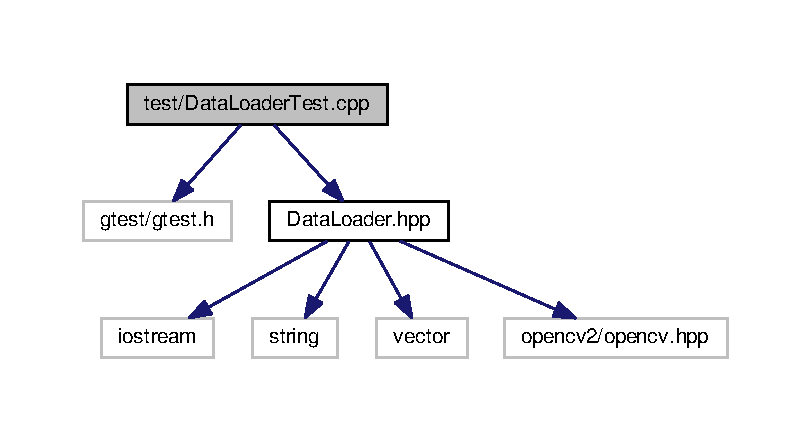
\includegraphics[width=350pt]{DataLoaderTest_8cpp__incl}
\end{center}
\end{figure}
\subsection*{Functions}
\begin{DoxyCompactItemize}
\item 
\hyperlink{DataLoaderTest_8cpp_a814ef08e5a582bb39ca1af2eb3d4ac8d}{T\+E\+ST} (Data\+Check, Check\+Images\+Read)\hypertarget{DataLoaderTest_8cpp_a814ef08e5a582bb39ca1af2eb3d4ac8d}{}\label{DataLoaderTest_8cpp_a814ef08e5a582bb39ca1af2eb3d4ac8d}

\begin{DoxyCompactList}\small\item\em Test for training data collection It checks whether \hyperlink{classDataLoader}{Data\+Loader} class is able to read images from given directory. \end{DoxyCompactList}\item 
\hyperlink{DataLoaderTest_8cpp_a5d3c64c2f5b8ff3c06b963f473c77576}{T\+E\+ST} (Data\+Check, Check\+Labels\+Created)\hypertarget{DataLoaderTest_8cpp_a5d3c64c2f5b8ff3c06b963f473c77576}{}\label{DataLoaderTest_8cpp_a5d3c64c2f5b8ff3c06b963f473c77576}

\begin{DoxyCompactList}\small\item\em Test for training labels creations It checks whether \hyperlink{classDataLoader}{Data\+Loader} class is able to generate labels for positive and negative images. \end{DoxyCompactList}\item 
\hyperlink{DataLoaderTest_8cpp_a2051b8b43279d7bf4c62de07426bfaef}{T\+E\+ST} (Data\+Check, Check\+Label\+Values)\hypertarget{DataLoaderTest_8cpp_a2051b8b43279d7bf4c62de07426bfaef}{}\label{DataLoaderTest_8cpp_a2051b8b43279d7bf4c62de07426bfaef}

\begin{DoxyCompactList}\small\item\em Test for training labels values It checks whether \hyperlink{classDataLoader}{Data\+Loader} class is able to generate right labels for positive and negative images. \end{DoxyCompactList}\item 
\hyperlink{DataLoaderTest_8cpp_aaaa38bf5225dd7727af448e19959eb4a}{T\+E\+ST} (Data\+Check, Check\+Empty)\hypertarget{DataLoaderTest_8cpp_aaaa38bf5225dd7727af448e19959eb4a}{}\label{DataLoaderTest_8cpp_aaaa38bf5225dd7727af448e19959eb4a}

\begin{DoxyCompactList}\small\item\em Test for non existing directory It checks the behaviour of \hyperlink{classDataLoader}{Data\+Loader} class with non existing directory. \end{DoxyCompactList}\end{DoxyCompactItemize}


\subsection{Detailed Description}
Test cases for \hyperlink{classDataLoader}{Data\+Loader} class methods. 

\begin{DoxyAuthor}{Author}
Saumil Shah (Saumil\+Shah66) Driver 

Naman Gupta (namangupta98) Navigator 

Aman Virmani (Aman\+Virmani) Design Keeper 
\end{DoxyAuthor}
\begin{DoxyCopyright}{Copyright}
M\+IT License 
\end{DoxyCopyright}

\hypertarget{DetectHumanTest_8cpp}{}\section{test/\+Detect\+Human\+Test.cpp File Reference}
\label{DetectHumanTest_8cpp}\index{test/\+Detect\+Human\+Test.\+cpp@{test/\+Detect\+Human\+Test.\+cpp}}


Test cases for \hyperlink{classVisionInput}{Vision\+Input} class methods.  


{\ttfamily \#include $<$gtest/gtest.\+h$>$}\\*
{\ttfamily \#include $<$stdio.\+h$>$}\\*
{\ttfamily \#include $<$Train\+S\+V\+M.\+hpp$>$}\\*
{\ttfamily \#include $<$opencv2/opencv.\+hpp$>$}\\*
{\ttfamily \#include $<$iostream$>$}\\*
{\ttfamily \#include $<$Detect\+Human.\+hpp$>$}\\*
Include dependency graph for Detect\+Human\+Test.\+cpp\+:
\nopagebreak
\begin{figure}[H]
\begin{center}
\leavevmode
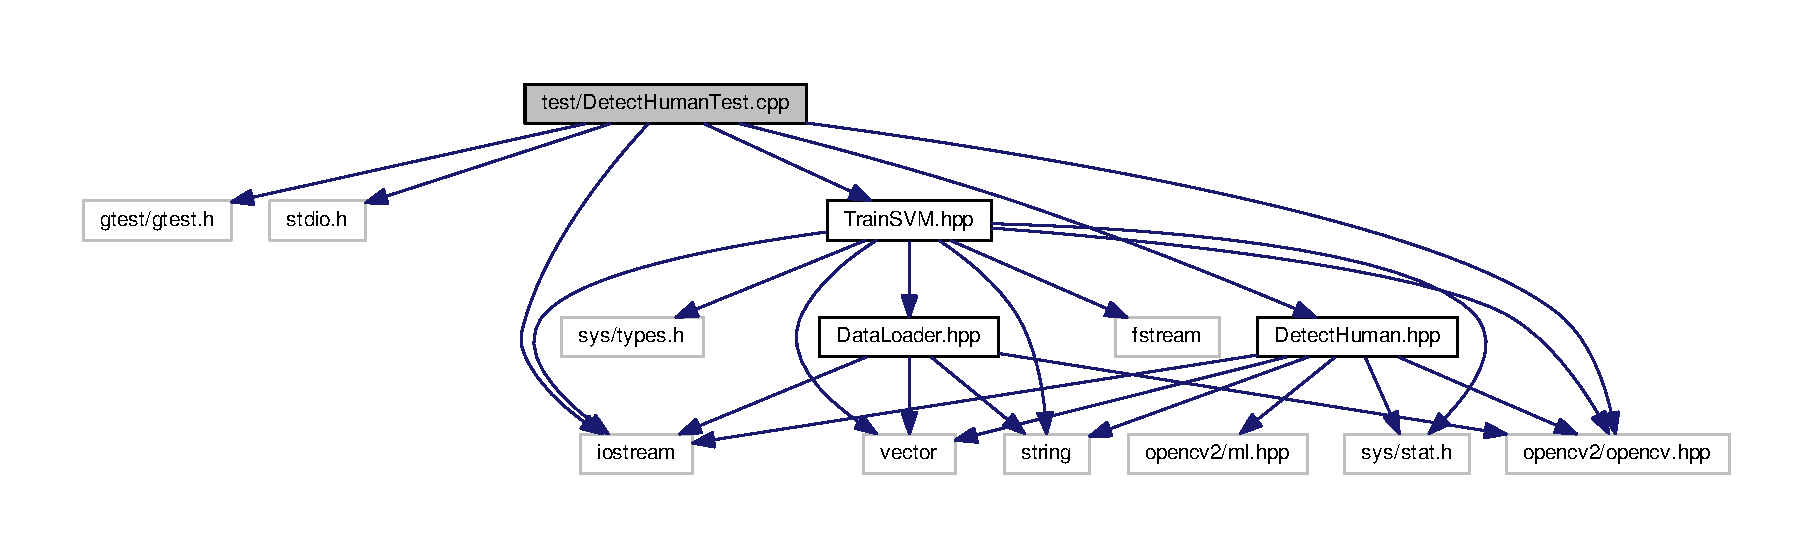
\includegraphics[width=350pt]{DetectHumanTest_8cpp__incl}
\end{center}
\end{figure}
\subsection*{Functions}
\begin{DoxyCompactItemize}
\item 
\hyperlink{DetectHumanTest_8cpp_a997a26dc0a06bfa70afa14e49aa1cc5f}{T\+E\+ST} (Detection\+Check, File\+Doesnot\+Exist)\hypertarget{DetectHumanTest_8cpp_a997a26dc0a06bfa70afa14e49aa1cc5f}{}\label{DetectHumanTest_8cpp_a997a26dc0a06bfa70afa14e49aa1cc5f}

\begin{DoxyCompactList}\small\item\em Test for \hyperlink{classDetectHuman}{Detect\+Human} class checks if file\+Exist methods works. \end{DoxyCompactList}\item 
\hyperlink{DetectHumanTest_8cpp_afa8daaea5e4c1081c0384741b61ff6b4}{T\+E\+ST} (Detection\+Check, File\+Exist)\hypertarget{DetectHumanTest_8cpp_afa8daaea5e4c1081c0384741b61ff6b4}{}\label{DetectHumanTest_8cpp_afa8daaea5e4c1081c0384741b61ff6b4}

\begin{DoxyCompactList}\small\item\em Test for \hyperlink{classDetectHuman}{Detect\+Human} class checks if file\+Exist methods works. \end{DoxyCompactList}\item 
\hyperlink{DetectHumanTest_8cpp_a4583578ffe7bc18f6a207424eef50425}{T\+E\+ST} (Detection\+Check, Reading\+Default\+S\+VM)\hypertarget{DetectHumanTest_8cpp_a4583578ffe7bc18f6a207424eef50425}{}\label{DetectHumanTest_8cpp_a4583578ffe7bc18f6a207424eef50425}

\begin{DoxyCompactList}\small\item\em Test for \hyperlink{classDetectHuman}{Detect\+Human} class checks if it sets default S\+VM. \end{DoxyCompactList}\item 
\hyperlink{DetectHumanTest_8cpp_adbb4521771baf97dad9a48b5a1f2224b}{T\+E\+ST} (Detection\+Check, Reading\+From\+Non\+Existing\+File)\hypertarget{DetectHumanTest_8cpp_adbb4521771baf97dad9a48b5a1f2224b}{}\label{DetectHumanTest_8cpp_adbb4521771baf97dad9a48b5a1f2224b}

\begin{DoxyCompactList}\small\item\em Test for \hyperlink{classDetectHuman}{Detect\+Human} class checks if it does not set S\+VM when passed file doesnot exist. \end{DoxyCompactList}\end{DoxyCompactItemize}


\subsection{Detailed Description}
Test cases for \hyperlink{classVisionInput}{Vision\+Input} class methods. 

\begin{DoxyAuthor}{Author}
Saumil Shah (Saumil\+Shah66) Driver 

Naman Gupta (namangupta98) Navigator 

Aman Virmani (Aman\+Virmani) Design Keeper 
\end{DoxyAuthor}
\begin{DoxyCopyright}{Copyright}
M\+IT License 
\end{DoxyCopyright}

\hypertarget{TrainSVMTest_8cpp}{}\section{test/\+Train\+S\+V\+M\+Test.cpp File Reference}
\label{TrainSVMTest_8cpp}\index{test/\+Train\+S\+V\+M\+Test.\+cpp@{test/\+Train\+S\+V\+M\+Test.\+cpp}}


Test cases for \hyperlink{classTrainSVM}{Train\+S\+VM} class methods.  


{\ttfamily \#include $<$gtest/gtest.\+h$>$}\\*
{\ttfamily \#include $<$stdio.\+h$>$}\\*
{\ttfamily \#include $<$Train\+S\+V\+M.\+hpp$>$}\\*
{\ttfamily \#include $<$opencv2/opencv.\+hpp$>$}\\*
{\ttfamily \#include $<$iostream$>$}\\*
Include dependency graph for Train\+S\+V\+M\+Test.\+cpp\+:
\nopagebreak
\begin{figure}[H]
\begin{center}
\leavevmode
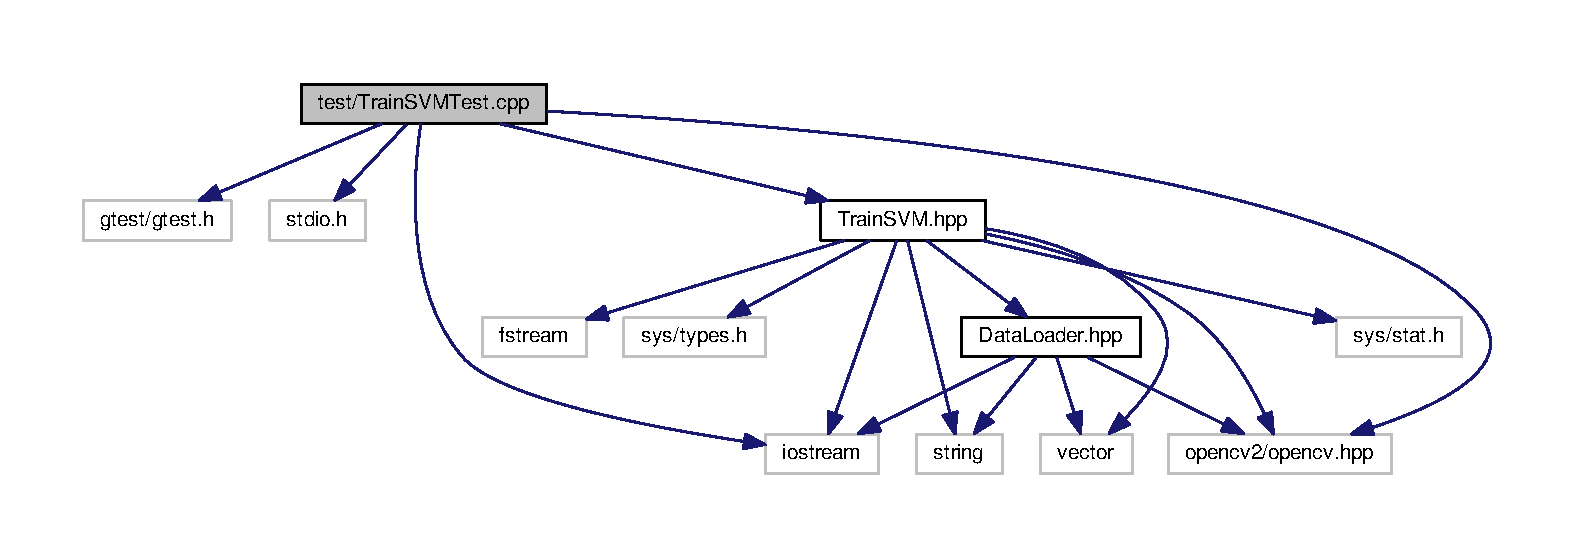
\includegraphics[width=350pt]{TrainSVMTest_8cpp__incl}
\end{center}
\end{figure}
\subsection*{Functions}
\begin{DoxyCompactItemize}
\item 
\hyperlink{TrainSVMTest_8cpp_acc53accfccca6a5d5fc1f8c8cbdf5817}{T\+E\+ST} (S\+V\+M\+Check, Should\+Not\+Train)\hypertarget{TrainSVMTest_8cpp_acc53accfccca6a5d5fc1f8c8cbdf5817}{}\label{TrainSVMTest_8cpp_acc53accfccca6a5d5fc1f8c8cbdf5817}

\begin{DoxyCompactList}\small\item\em Test for S\+VM training It checks S\+V\+M\+Trainer class must not train with empty given directory. \end{DoxyCompactList}\item 
\hyperlink{TrainSVMTest_8cpp_ae6b9d4f76413df93ceb0cb737f8b9b3c}{T\+E\+ST} (S\+V\+M\+Check, Should\+Train)\hypertarget{TrainSVMTest_8cpp_ae6b9d4f76413df93ceb0cb737f8b9b3c}{}\label{TrainSVMTest_8cpp_ae6b9d4f76413df93ceb0cb737f8b9b3c}

\begin{DoxyCompactList}\small\item\em Test for S\+VM training It checks whether S\+V\+M\+Trainer class has trained a classifier and saved it or not. \end{DoxyCompactList}\end{DoxyCompactItemize}


\subsection{Detailed Description}
Test cases for \hyperlink{classTrainSVM}{Train\+S\+VM} class methods. 

\begin{DoxyAuthor}{Author}
Saumil Shah (Saumil\+Shah66) Driver 

Naman Gupta (namangupta98) Navigator 

Aman Virmani (Aman\+Virmani) Design Keeper 
\end{DoxyAuthor}
\begin{DoxyCopyright}{Copyright}
M\+IT License 
\end{DoxyCopyright}

\hypertarget{VisionInputTest_8cpp}{}\section{test/\+Vision\+Input\+Test.cpp File Reference}
\label{VisionInputTest_8cpp}\index{test/\+Vision\+Input\+Test.\+cpp@{test/\+Vision\+Input\+Test.\+cpp}}


Test cases for \hyperlink{classVisionInput}{Vision\+Input} class methods.  


{\ttfamily \#include $<$gtest/gtest.\+h$>$}\\*
{\ttfamily \#include $<$stdio.\+h$>$}\\*
{\ttfamily \#include $<$Train\+S\+V\+M.\+hpp$>$}\\*
{\ttfamily \#include $<$opencv2/opencv.\+hpp$>$}\\*
{\ttfamily \#include $<$iostream$>$}\\*
{\ttfamily \#include $<$Vision\+Input.\+hpp$>$}\\*
Include dependency graph for Vision\+Input\+Test.\+cpp\+:
\nopagebreak
\begin{figure}[H]
\begin{center}
\leavevmode
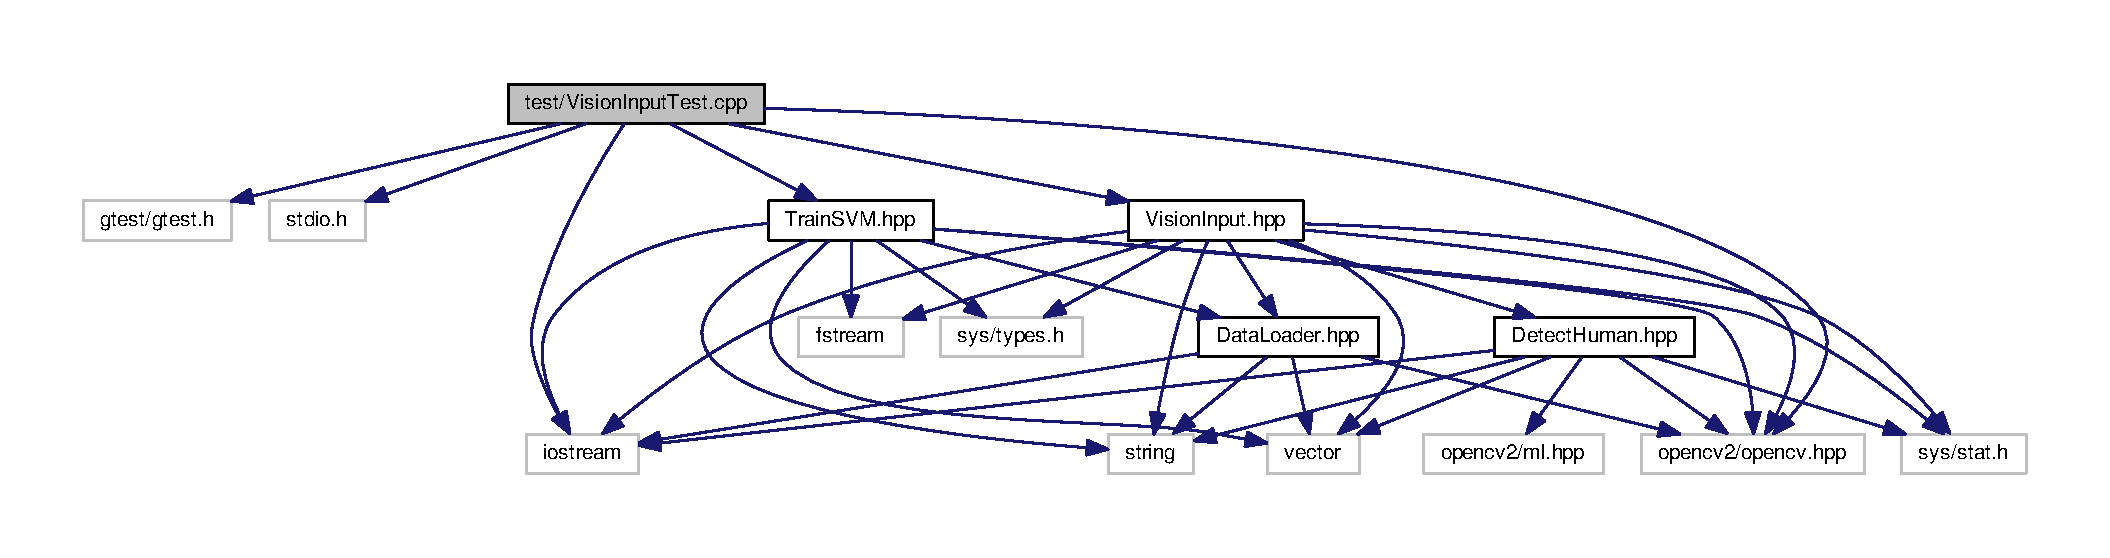
\includegraphics[width=350pt]{VisionInputTest_8cpp__incl}
\end{center}
\end{figure}
\subsection*{Functions}
\begin{DoxyCompactItemize}
\item 
\hyperlink{VisionInputTest_8cpp_ae3df2e09352021c28a4f0ac7e644357a}{T\+E\+ST} (Camera\+Check, No\+Present\+Camera\+Check)\hypertarget{VisionInputTest_8cpp_ae3df2e09352021c28a4f0ac7e644357a}{}\label{VisionInputTest_8cpp_ae3df2e09352021c28a4f0ac7e644357a}

\begin{DoxyCompactList}\small\item\em Test for camera sensor read when no camera is present It checks whether image container of class object is empty or not in order to make sure it is not reading any data as no camera is present. \end{DoxyCompactList}\item 
\hyperlink{VisionInputTest_8cpp_a324a9d79633517a48e3722ad7f6f1ed2}{T\+E\+ST} (Video\+File\+Check, Should\+Read\+Frames)\hypertarget{VisionInputTest_8cpp_a324a9d79633517a48e3722ad7f6f1ed2}{}\label{VisionInputTest_8cpp_a324a9d79633517a48e3722ad7f6f1ed2}

\begin{DoxyCompactList}\small\item\em Test for checking video file read It checks whether \hyperlink{classVisionInput}{Vision\+Input} class is able to parse frames from specified video file. \end{DoxyCompactList}\item 
\hyperlink{VisionInputTest_8cpp_a49bba036c4226a2652b63206b74f5621}{T\+E\+ST} (Video\+File\+Check, No\+Video\+File)\hypertarget{VisionInputTest_8cpp_a49bba036c4226a2652b63206b74f5621}{}\label{VisionInputTest_8cpp_a49bba036c4226a2652b63206b74f5621}

\begin{DoxyCompactList}\small\item\em Test for checking empty video file read Program should not crash if non existing files are passed to read. \end{DoxyCompactList}\item 
\hyperlink{VisionInputTest_8cpp_a778c96651540193802d5ce6879809b08}{T\+E\+ST} (Image\+File\+Check, Image\+Read\+Successfully)\hypertarget{VisionInputTest_8cpp_a778c96651540193802d5ce6879809b08}{}\label{VisionInputTest_8cpp_a778c96651540193802d5ce6879809b08}

\begin{DoxyCompactList}\small\item\em Test for reading image from file Checksif object is able to read imagefile succesfully. \end{DoxyCompactList}\item 
\hyperlink{VisionInputTest_8cpp_ae1b7acc1c4a20953856285c188172651}{T\+E\+ST} (Image\+File\+Check, Non\+Existing\+File)\hypertarget{VisionInputTest_8cpp_ae1b7acc1c4a20953856285c188172651}{}\label{VisionInputTest_8cpp_ae1b7acc1c4a20953856285c188172651}

\begin{DoxyCompactList}\small\item\em Test for reading image from non existing file Programe should not crash if file is not available. \end{DoxyCompactList}\end{DoxyCompactItemize}


\subsection{Detailed Description}
Test cases for \hyperlink{classVisionInput}{Vision\+Input} class methods. 

\begin{DoxyAuthor}{Author}
Saumil Shah (Saumil\+Shah66) Driver 

Naman Gupta (namangupta98) Navigator 

Aman Virmani (Aman\+Virmani) Design Keeper 
\end{DoxyAuthor}
\begin{DoxyCopyright}{Copyright}
M\+IT License 
\end{DoxyCopyright}

%--- End generated contents ---

% Index
\backmatter
\newpage
\phantomsection
\clearemptydoublepage
\addcontentsline{toc}{chapter}{Index}
\printindex

\end{document}
